\documentclass[twoside]{book}

% Packages required by doxygen
\usepackage{fixltx2e}
\usepackage{calc}
\usepackage{doxygen}
\usepackage[export]{adjustbox} % also loads graphicx
\usepackage{graphicx}
\usepackage[utf8]{inputenc}
\usepackage{makeidx}
\usepackage{multicol}
\usepackage{multirow}
\PassOptionsToPackage{warn}{textcomp}
\usepackage{textcomp}
\usepackage[nointegrals]{wasysym}
\usepackage[table]{xcolor}

% NLS support packages
\usepackage[catalan]{babel}

% Font selection
\usepackage[T1]{fontenc}
\usepackage[scaled=.90]{helvet}
\usepackage{courier}
\usepackage{amssymb}
\usepackage{sectsty}
\renewcommand{\familydefault}{\sfdefault}
\allsectionsfont{%
  \fontseries{bc}\selectfont%
  \color{darkgray}%
}
\renewcommand{\DoxyLabelFont}{%
  \fontseries{bc}\selectfont%
  \color{darkgray}%
}
\newcommand{\+}{\discretionary{\mbox{\scriptsize$\hookleftarrow$}}{}{}}

% Page & text layout
\usepackage{geometry}
\geometry{%
  a4paper,%
  top=2.5cm,%
  bottom=2.5cm,%
  left=2.5cm,%
  right=2.5cm%
}
\tolerance=750
\hfuzz=15pt
\hbadness=750
\setlength{\emergencystretch}{15pt}
\setlength{\parindent}{0cm}
\setlength{\parskip}{3ex plus 2ex minus 2ex}
\makeatletter
\renewcommand{\paragraph}{%
  \@startsection{paragraph}{4}{0ex}{-1.0ex}{1.0ex}{%
    \normalfont\normalsize\bfseries\SS@parafont%
  }%
}
\renewcommand{\subparagraph}{%
  \@startsection{subparagraph}{5}{0ex}{-1.0ex}{1.0ex}{%
    \normalfont\normalsize\bfseries\SS@subparafont%
  }%
}
\makeatother

% Headers & footers
\usepackage{fancyhdr}
\pagestyle{fancyplain}
\fancyhead[LE]{\fancyplain{}{\bfseries\thepage}}
\fancyhead[CE]{\fancyplain{}{}}
\fancyhead[RE]{\fancyplain{}{\bfseries\leftmark}}
\fancyhead[LO]{\fancyplain{}{\bfseries\rightmark}}
\fancyhead[CO]{\fancyplain{}{}}
\fancyhead[RO]{\fancyplain{}{\bfseries\thepage}}
\fancyfoot[LE]{\fancyplain{}{}}
\fancyfoot[CE]{\fancyplain{}{}}
\fancyfoot[RE]{\fancyplain{}{\bfseries\scriptsize Generat per Doxygen }}
\fancyfoot[LO]{\fancyplain{}{\bfseries\scriptsize Generat per Doxygen }}
\fancyfoot[CO]{\fancyplain{}{}}
\fancyfoot[RO]{\fancyplain{}{}}
\renewcommand{\footrulewidth}{0.4pt}
\renewcommand{\chaptermark}[1]{%
  \markboth{#1}{}%
}
\renewcommand{\sectionmark}[1]{%
  \markright{\thesection\ #1}%
}

% Indices & bibliography
\usepackage{natbib}
\usepackage[titles]{tocloft}
\setcounter{tocdepth}{3}
\setcounter{secnumdepth}{5}
\makeindex

% Hyperlinks (required, but should be loaded last)
\usepackage{ifpdf}
\ifpdf
  \usepackage[pdftex,pagebackref=true]{hyperref}
\else
  \usepackage[ps2pdf,pagebackref=true]{hyperref}
\fi
\hypersetup{%
  colorlinks=true,%
  linkcolor=blue,%
  citecolor=blue,%
  unicode%
}

% Custom commands
\newcommand{\clearemptydoublepage}{%
  \newpage{\pagestyle{empty}\cleardoublepage}%
}

\usepackage{caption}
\captionsetup{labelsep=space,justification=centering,font={bf},singlelinecheck=off,skip=4pt,position=top}

%===== C O N T E N T S =====

\begin{document}

% Titlepage & ToC
\hypersetup{pageanchor=false,
             bookmarksnumbered=true,
             pdfencoding=unicode
            }
\pagenumbering{roman}
\begin{titlepage}
\vspace*{7cm}
\begin{center}%
{\Large Albert Pita Argemi. Practica de P\+R\+O2. Tree\+K\+EA. \\[1ex]\large v2.\+0 29-\/05-\/2018 }\\
\vspace*{1cm}
{\large Generat per Doxygen 1.8.11}\\
\end{center}
\end{titlepage}
\clearemptydoublepage
\tableofcontents
\clearemptydoublepage
\pagenumbering{arabic}
\hypersetup{pageanchor=true}

%--- Begin generated contents ---
\chapter{Tree\+K\+EA, simulacio d\textquotesingle{}un nou model de magatzem.}
\label{index}\hypertarget{index}{}Una cadena de tendes de mobles vol cambiar els seus metodes d\textquotesingle{}emmagatzematge provant noves distribucions als seus magatzems. I ens han encarregat que implementem una simulacio del nou tipus de magatzem per poder estudiar si adapten o no aquest nou diseny en futures tendes.

En aquest programa s\textquotesingle{}introdueixen les classes {\itshape \hyperlink{class_magatzem}{Magatzem}}, {\itshape \hyperlink{class_estanteria}{Estanteria}} i {\itshape \hyperlink{class_sistema}{Sistema}}.

Fet per Albert Pita Argemi. 
\chapter{Índex de Classes}
\section{Llista de Classes}
Aquestes són les classes, estructures, unions i interfícies acompanyades amb breus descripcions\+:\begin{DoxyCompactList}
\item\contentsline{section}{\hyperlink{class_estanteria}{Estanteria} \\*Representa l\textquotesingle{}estanteria que hi ha a cada sala }{\pageref{class_estanteria}}{}
\item\contentsline{section}{\hyperlink{class_magatzem}{Magatzem} \\*Representa un magatzem }{\pageref{class_magatzem}}{}
\item\contentsline{section}{\hyperlink{class_sistema}{Sistema} \\*Representa el sistema que controla els productes que hi ha dins del magatzem }{\pageref{class_sistema}}{}
\end{DoxyCompactList}

\chapter{Índex de Fitxers}
\section{Llista dels Fitxers}
Aquesta és la llista de tots els fitxers acompanyats amb breus descripcions\+:\begin{DoxyCompactList}
\item\contentsline{section}{\hyperlink{_estanteria_8cc}{Estanteria.\+cc} }{\pageref{_estanteria_8cc}}{}
\item\contentsline{section}{\hyperlink{_estanteria_8hh}{Estanteria.\+hh} \\*Especificacio de la classe \hyperlink{class_estanteria}{Estanteria} }{\pageref{_estanteria_8hh}}{}
\item\contentsline{section}{\hyperlink{_magatzem_8cc}{Magatzem.\+cc} }{\pageref{_magatzem_8cc}}{}
\item\contentsline{section}{\hyperlink{_magatzem_8hh}{Magatzem.\+hh} \\*Especificacio de la classe \hyperlink{class_magatzem}{Magatzem} }{\pageref{_magatzem_8hh}}{}
\item\contentsline{section}{\hyperlink{program_8cc}{program.\+cc} }{\pageref{program_8cc}}{}
\item\contentsline{section}{\hyperlink{_sistema_8cc}{Sistema.\+cc} \\*Codi de la classe \hyperlink{_sistema_8cc}{Sistema.\+cc} }{\pageref{_sistema_8cc}}{}
\item\contentsline{section}{\hyperlink{_sistema_8hh}{Sistema.\+hh} \\*Especificacio de la classe \hyperlink{class_sistema}{Sistema} }{\pageref{_sistema_8hh}}{}
\end{DoxyCompactList}

\chapter{Documentació de les Classes}
\hypertarget{class_estanteria}{}\section{Referència de la Classe Estanteria}
\label{class_estanteria}\index{Estanteria@{Estanteria}}


Representa l\textquotesingle{}estanteria que hi ha a cada sala.  


\subsection*{Mètodes públics}
\begin{DoxyCompactItemize}
\item 
\hyperlink{class_estanteria_a55c7a4e067b17ba7e79f61ce8929ac88}{Estanteria} ()
\begin{DoxyCompactList}\small\item\em Creadora per defecte. \end{DoxyCompactList}\item 
\hyperlink{class_estanteria_ab0593879a794013eb05ee0b3b61dfd54}{Estanteria} (int i, int j)
\begin{DoxyCompactList}\small\item\em Constructora que crea una estanteria de mida ixj. \end{DoxyCompactList}\item 
\hyperlink{class_estanteria_a4d7827dbb58db685a34b305b6ff8e755}{$\sim$\+Estanteria} ()
\begin{DoxyCompactList}\small\item\em Destructora per defecte. Esborra automàticament els objectes locals en sortir d\textquotesingle{}un àmbit de visibilitat. \end{DoxyCompactList}\item 
int \hyperlink{class_estanteria_a8ab96b52673441f441cec50fb8e9378e}{afegir\+\_\+producte} (string \&idprod, int quantitat)
\begin{DoxyCompactList}\small\item\em Coloca una certa quantitat d\textquotesingle{}un mateix producte dins del parametre implicit(una estanteria). \end{DoxyCompactList}\item 
int \hyperlink{class_estanteria_a19a5ab5427f1ded37722fc071e87ef41}{eliminar\+\_\+productes} (string \&idprod, int quantitat)
\begin{DoxyCompactList}\small\item\em Elimina una certa quantitat d\textquotesingle{}un mateix producte dins del parametre implicit(una estanteria). \end{DoxyCompactList}\item 
void \hyperlink{class_estanteria_aefcf5c93b909a2d61c5805c4e39f56d1}{compactar\+\_\+estanteria} ()
\begin{DoxyCompactList}\small\item\em Es realitza la compactacio del parametre implicit. \end{DoxyCompactList}\item 
void \hyperlink{class_estanteria_a605404d278df85704686201e9ac5bc4b}{reorganitzar\+\_\+estanteria} ()
\begin{DoxyCompactList}\small\item\em Es realitza la reorganització del parametre implicit. \end{DoxyCompactList}\item 
void \hyperlink{class_estanteria_a4a5f0fb1576fc6245bd81249fedb2bb4}{Estanteria\+\_\+redimensionada} (int i, int j)
\begin{DoxyCompactList}\small\item\em Si totes les unitats dels productes que te el parametre implicit $<$= ixj, la nova dimensio de l\textquotesingle{}estanteria sera ixj. \end{DoxyCompactList}\item 
bool \hyperlink{class_estanteria_a28210da5d76be58356c3544871130a2e}{no\+\_\+buida} ()
\begin{DoxyCompactList}\small\item\em Retorna un boolea que diu si el parametre implicit esta buit o no. \end{DoxyCompactList}\item 
string \hyperlink{class_estanteria_ad0b776e636062653f986010880610ced}{consultar\+\_\+pos\+\_\+estanteria} (int i, int j)
\begin{DoxyCompactList}\small\item\em Indica quin producte hi ha a la posicio (i,j) del parametre implicit. \end{DoxyCompactList}\item 
void \hyperlink{class_estanteria_ac00f0367653416ca3bd588939a7c9c22}{escriure\+\_\+estanteria} () const 
\begin{DoxyCompactList}\small\item\em Escriu per pantalla el parametre implicit. \end{DoxyCompactList}\end{DoxyCompactItemize}
\subsection*{Atributs Privats}
\begin{DoxyCompactItemize}
\item 
int \hyperlink{class_estanteria_a649ad0331b78ba3c056fd9c42f0d26fe}{files}
\begin{DoxyCompactList}\small\item\em Files de l\textquotesingle{}estanteria. \end{DoxyCompactList}\item 
int \hyperlink{class_estanteria_afd7a5087a18c8481060aef57ca8cbf78}{columnes}
\begin{DoxyCompactList}\small\item\em Columnes de l\textquotesingle{}estanteria. \end{DoxyCompactList}\item 
vector$<$ string $>$ \hyperlink{class_estanteria_a4ed61c91fcad6b38af067a4be8233097}{Est}
\begin{DoxyCompactList}\small\item\em Estructura de l\textquotesingle{}estanteria. \end{DoxyCompactList}\item 
map$<$ string, int $>$ \hyperlink{class_estanteria_af37488895058b4673e3d093a84df4c63}{inv\+\_\+sala}
\begin{DoxyCompactList}\small\item\em Inventari de la sala. \end{DoxyCompactList}\end{DoxyCompactItemize}


\subsection{Descripció Detallada}
Representa l\textquotesingle{}estanteria que hi ha a cada sala. 

Te un tamany ixj. Pot contindre en cada una de les seves caselles o un producte o res (representat amb la paraula N\+U\+LL). S\textquotesingle{}utilitza per emmagatzemar productes. Es poden afegir productes o eliminar-\/los. Es pot reordenar de dues formes diferents, compactant l\textquotesingle{}estanteria o reorganitzant-\/la. També es possible redimensionar l\textquotesingle{}estanteria donant un nou tamany si aquest compleix certes condicions. També es pot consultar que hi ha en una posicio especifica d\textquotesingle{}ella. 

Definició a la línia 28 del fitxer Estanteria.\+hh.



\subsection{Documentació del Constructor i el Destructor}
\index{Estanteria@{Estanteria}!Estanteria@{Estanteria}}
\index{Estanteria@{Estanteria}!Estanteria@{Estanteria}}
\subsubsection[{\texorpdfstring{Estanteria()}{Estanteria()}}]{\setlength{\rightskip}{0pt plus 5cm}Estanteria\+::\+Estanteria (
\begin{DoxyParamCaption}
{}
\end{DoxyParamCaption}
)}\hypertarget{class_estanteria_a55c7a4e067b17ba7e79f61ce8929ac88}{}\label{class_estanteria_a55c7a4e067b17ba7e79f61ce8929ac88}


Creadora per defecte. 

Se executa automaticament al declarar una estanteria. \begin{DoxyPrecond}{Precondició}
{\itshape cert} 
\end{DoxyPrecond}
\begin{DoxyPostcond}{Postcondició}
Crea una estanteria de 0x0 buida 
\end{DoxyPostcond}


Definició a la línia 3 del fitxer Estanteria.\+cc.


\begin{DoxyCode}
3                        \{
4     \hyperlink{class_estanteria_a4ed61c91fcad6b38af067a4be8233097}{Est} = (vector<string>(0));
5     \hyperlink{class_estanteria_a649ad0331b78ba3c056fd9c42f0d26fe}{files} = 0;
6     \hyperlink{class_estanteria_afd7a5087a18c8481060aef57ca8cbf78}{columnes} = 0;
7 \}
\end{DoxyCode}
\index{Estanteria@{Estanteria}!Estanteria@{Estanteria}}
\index{Estanteria@{Estanteria}!Estanteria@{Estanteria}}
\subsubsection[{\texorpdfstring{Estanteria(int i, int j)}{Estanteria(int i, int j)}}]{\setlength{\rightskip}{0pt plus 5cm}Estanteria\+::\+Estanteria (
\begin{DoxyParamCaption}
\item[{int}]{i, }
\item[{int}]{j}
\end{DoxyParamCaption}
)}\hypertarget{class_estanteria_ab0593879a794013eb05ee0b3b61dfd54}{}\label{class_estanteria_ab0593879a794013eb05ee0b3b61dfd54}


Constructora que crea una estanteria de mida ixj. 

Permet declarar una estanteria nova de {\itshape i} files i {\itshape j} columnes. \begin{DoxyPrecond}{Precondició}
i $>$= 1 i j $>$= 1 
\end{DoxyPrecond}
\begin{DoxyPostcond}{Postcondició}
Crea una estanteria de i files amb j columnes plena de productes nuls 
\end{DoxyPostcond}


Definició a la línia 9 del fitxer Estanteria.\+cc.


\begin{DoxyCode}
9                                    \{
10     \hyperlink{class_estanteria_a4ed61c91fcad6b38af067a4be8233097}{Est} = (vector<string> (i*j));
11     \hyperlink{class_estanteria_a649ad0331b78ba3c056fd9c42f0d26fe}{files} = i;
12     \hyperlink{class_estanteria_afd7a5087a18c8481060aef57ca8cbf78}{columnes} = j;
13 \}
\end{DoxyCode}
\index{Estanteria@{Estanteria}!````~Estanteria@{$\sim$\+Estanteria}}
\index{````~Estanteria@{$\sim$\+Estanteria}!Estanteria@{Estanteria}}
\subsubsection[{\texorpdfstring{$\sim$\+Estanteria()}{~Estanteria()}}]{\setlength{\rightskip}{0pt plus 5cm}Estanteria\+::$\sim$\+Estanteria (
\begin{DoxyParamCaption}
{}
\end{DoxyParamCaption}
)}\hypertarget{class_estanteria_a4d7827dbb58db685a34b305b6ff8e755}{}\label{class_estanteria_a4d7827dbb58db685a34b305b6ff8e755}


Destructora per defecte. Esborra automàticament els objectes locals en sortir d\textquotesingle{}un àmbit de visibilitat. 

\begin{DoxyPrecond}{Precondició}
Existeix una estanteria 
\end{DoxyPrecond}
\begin{DoxyPostcond}{Postcondició}
Destrueix la estanteria 
\end{DoxyPostcond}


Definició a la línia 15 del fitxer Estanteria.\+cc.


\begin{DoxyCode}
15 \{\}
\end{DoxyCode}


\subsection{Documentació de les Funcions Membre}
\index{Estanteria@{Estanteria}!afegir\+\_\+producte@{afegir\+\_\+producte}}
\index{afegir\+\_\+producte@{afegir\+\_\+producte}!Estanteria@{Estanteria}}
\subsubsection[{\texorpdfstring{afegir\+\_\+producte(string \&idprod, int quantitat)}{afegir_producte(string &idprod, int quantitat)}}]{\setlength{\rightskip}{0pt plus 5cm}int Estanteria\+::afegir\+\_\+producte (
\begin{DoxyParamCaption}
\item[{string \&}]{idprod, }
\item[{int}]{quantitat}
\end{DoxyParamCaption}
)}\hypertarget{class_estanteria_a8ab96b52673441f441cec50fb8e9378e}{}\label{class_estanteria_a8ab96b52673441f441cec50fb8e9378e}


Coloca una certa quantitat d\textquotesingle{}un mateix producte dins del parametre implicit(una estanteria). 

\begin{DoxyPrecond}{Precondició}
Al canal estandard d\textquotesingle{}entrada hi ha preparades l\textquotesingle{}identificador d\textquotesingle{}un producte i una certa quantitat 
\end{DoxyPrecond}
\begin{DoxyPostcond}{Postcondició}
S\textquotesingle{}afegeixen totes les unitats(= quantitat) que entrin dins el parametre implicit i es retorna la quantitat que no s\textquotesingle{}ha pogut afegir 
\end{DoxyPostcond}


Definició a la línia 17 del fitxer Estanteria.\+cc.


\begin{DoxyCode}
17                                                              \{
18     \textcolor{keywordtype}{int} aux = quantitat;
19     \textcolor{keywordtype}{bool} ha\_afegit = \textcolor{keyword}{false};
20     \textcolor{keywordflow}{for} (\textcolor{keywordtype}{int} i = 0; i < \hyperlink{class_estanteria_a4ed61c91fcad6b38af067a4be8233097}{Est}.size() and quantitat > 0; ++i) \{
21         \textcolor{keywordflow}{if} (\hyperlink{class_estanteria_a4ed61c91fcad6b38af067a4be8233097}{Est}[i] == \textcolor{stringliteral}{""}) \{
22             \hyperlink{class_estanteria_a4ed61c91fcad6b38af067a4be8233097}{Est}[i] = idprod;
23             --quantitat;
24             ha\_afegit = \textcolor{keyword}{true};
25         \}
26     \}
27     \textcolor{keywordflow}{if} (ha\_afegit) \{
28         map<string,int>::iterator it = \hyperlink{class_estanteria_af37488895058b4673e3d093a84df4c63}{inv\_sala}.find(idprod);
29         \textcolor{keywordflow}{if} (it != \hyperlink{class_estanteria_af37488895058b4673e3d093a84df4c63}{inv\_sala}.end()) it->second += (aux-quantitat);
30         \textcolor{keywordflow}{else} \{
31             pair<string,int> x;
32             x.first = idprod;
33             x.second = (aux-quantitat);
34             \hyperlink{class_estanteria_af37488895058b4673e3d093a84df4c63}{inv\_sala}.insert(x);
35         \}
36     \}
37     \textcolor{keywordflow}{return} quantitat;
38 \}
\end{DoxyCode}
\index{Estanteria@{Estanteria}!eliminar\+\_\+productes@{eliminar\+\_\+productes}}
\index{eliminar\+\_\+productes@{eliminar\+\_\+productes}!Estanteria@{Estanteria}}
\subsubsection[{\texorpdfstring{eliminar\+\_\+productes(string \&idprod, int quantitat)}{eliminar_productes(string &idprod, int quantitat)}}]{\setlength{\rightskip}{0pt plus 5cm}int Estanteria\+::eliminar\+\_\+productes (
\begin{DoxyParamCaption}
\item[{string \&}]{idprod, }
\item[{int}]{quantitat}
\end{DoxyParamCaption}
)}\hypertarget{class_estanteria_a19a5ab5427f1ded37722fc071e87ef41}{}\label{class_estanteria_a19a5ab5427f1ded37722fc071e87ef41}


Elimina una certa quantitat d\textquotesingle{}un mateix producte dins del parametre implicit(una estanteria). 

\begin{DoxyPrecond}{Precondició}
Al canal estandard d\textquotesingle{}entrada hi ha preparades l\textquotesingle{}identificador d\textquotesingle{}un producte i una certa quantitat 
\end{DoxyPrecond}
\begin{DoxyPostcond}{Postcondició}
S\textquotesingle{}eliminen totes les unitats(= quantitat) del parametre implicit amb identificador = {\itshape idprod} i es retorna la quantitat que no s\textquotesingle{}ha pogut eliminar 
\end{DoxyPostcond}


Definició a la línia 40 del fitxer Estanteria.\+cc.


\begin{DoxyCode}
40                                                                \{
41     \textcolor{keywordtype}{int} aux = quantitat;
42     \textcolor{keywordtype}{bool} ha\_borrat = \textcolor{keyword}{false};
43     \textcolor{keywordflow}{for} (\textcolor{keywordtype}{int} i = 0; i < \hyperlink{class_estanteria_a4ed61c91fcad6b38af067a4be8233097}{Est}.size() and quantitat > 0; ++i) \{
44         \textcolor{keywordflow}{if} (\hyperlink{class_estanteria_a4ed61c91fcad6b38af067a4be8233097}{Est}[i] == idprod) \{
45             \hyperlink{class_estanteria_a4ed61c91fcad6b38af067a4be8233097}{Est}[i] = \textcolor{stringliteral}{""};
46             --quantitat;
47             ha\_borrat = \textcolor{keyword}{true};
48         \}
49     \}
50     \textcolor{keywordflow}{if} (ha\_borrat) \{
51         map<string,int>::iterator it = \hyperlink{class_estanteria_af37488895058b4673e3d093a84df4c63}{inv\_sala}.find(idprod);
52         it->second -= (aux-quantitat);
53         \textcolor{keywordflow}{if} (it->second == 0) \hyperlink{class_estanteria_af37488895058b4673e3d093a84df4c63}{inv\_sala}.erase(idprod);
54     \}
55     \textcolor{keywordflow}{return} quantitat;
56 \}
\end{DoxyCode}
\index{Estanteria@{Estanteria}!compactar\+\_\+estanteria@{compactar\+\_\+estanteria}}
\index{compactar\+\_\+estanteria@{compactar\+\_\+estanteria}!Estanteria@{Estanteria}}
\subsubsection[{\texorpdfstring{compactar\+\_\+estanteria()}{compactar_estanteria()}}]{\setlength{\rightskip}{0pt plus 5cm}void Estanteria\+::compactar\+\_\+estanteria (
\begin{DoxyParamCaption}
{}
\end{DoxyParamCaption}
)}\hypertarget{class_estanteria_aefcf5c93b909a2d61c5805c4e39f56d1}{}\label{class_estanteria_aefcf5c93b909a2d61c5805c4e39f56d1}


Es realitza la compactacio del parametre implicit. 

\begin{DoxyPrecond}{Precondició}
{\itshape cert} 
\end{DoxyPrecond}
\begin{DoxyPostcond}{Postcondició}
Els productes queden compactats cap a l\textquotesingle{}esquerra i cap a baix de manera que no quedi cap forat entre dos productes 
\end{DoxyPostcond}


Definició a la línia 58 del fitxer Estanteria.\+cc.


\begin{DoxyCode}
58                                       \{
59     \textcolor{keywordtype}{int} poscanvi = 0;
60     \textcolor{keywordtype}{bool} canvi = \textcolor{keyword}{false};
61     \textcolor{keywordflow}{for} (\textcolor{keywordtype}{int} i = 0; i < \hyperlink{class_estanteria_a4ed61c91fcad6b38af067a4be8233097}{Est}.size(); ++i) \{
62         \textcolor{keywordflow}{if} (\hyperlink{class_estanteria_a4ed61c91fcad6b38af067a4be8233097}{Est}[i] == \textcolor{stringliteral}{""} and not canvi) \{
63             canvi = \textcolor{keyword}{true};
64             poscanvi = i;
65         \}
66         \textcolor{keywordflow}{else} \textcolor{keywordflow}{if} (\hyperlink{class_estanteria_a4ed61c91fcad6b38af067a4be8233097}{Est}[i] != \textcolor{stringliteral}{""} and canvi)\{
67             swap(\hyperlink{class_estanteria_a4ed61c91fcad6b38af067a4be8233097}{Est}[poscanvi],\hyperlink{class_estanteria_a4ed61c91fcad6b38af067a4be8233097}{Est}[i]);
68             canvi = \textcolor{keyword}{false};
69             i = poscanvi;
70         \}
71     \}
72 \}
\end{DoxyCode}
\index{Estanteria@{Estanteria}!reorganitzar\+\_\+estanteria@{reorganitzar\+\_\+estanteria}}
\index{reorganitzar\+\_\+estanteria@{reorganitzar\+\_\+estanteria}!Estanteria@{Estanteria}}
\subsubsection[{\texorpdfstring{reorganitzar\+\_\+estanteria()}{reorganitzar_estanteria()}}]{\setlength{\rightskip}{0pt plus 5cm}void Estanteria\+::reorganitzar\+\_\+estanteria (
\begin{DoxyParamCaption}
{}
\end{DoxyParamCaption}
)}\hypertarget{class_estanteria_a605404d278df85704686201e9ac5bc4b}{}\label{class_estanteria_a605404d278df85704686201e9ac5bc4b}


Es realitza la reorganització del parametre implicit. 

\begin{DoxyPrecond}{Precondició}
{\itshape cert} 
\end{DoxyPrecond}
\begin{DoxyPostcond}{Postcondició}
Els productes queden reorganitzats alfabèticament sense deixar espais ni abans ni entre ells 
\end{DoxyPostcond}


Definició a la línia 81 del fitxer Estanteria.\+cc.


\begin{DoxyCode}
81                                          \{
82     sort(\hyperlink{class_estanteria_a4ed61c91fcad6b38af067a4be8233097}{Est}.begin(),\hyperlink{class_estanteria_a4ed61c91fcad6b38af067a4be8233097}{Est}.end(),\hyperlink{_estanteria_8cc_ac0047e8b44c74d982f8a9009e43c3e96}{cmp});
83 \}
\end{DoxyCode}
\index{Estanteria@{Estanteria}!Estanteria\+\_\+redimensionada@{Estanteria\+\_\+redimensionada}}
\index{Estanteria\+\_\+redimensionada@{Estanteria\+\_\+redimensionada}!Estanteria@{Estanteria}}
\subsubsection[{\texorpdfstring{Estanteria\+\_\+redimensionada(int i, int j)}{Estanteria_redimensionada(int i, int j)}}]{\setlength{\rightskip}{0pt plus 5cm}void Estanteria\+::\+Estanteria\+\_\+redimensionada (
\begin{DoxyParamCaption}
\item[{int}]{i, }
\item[{int}]{j}
\end{DoxyParamCaption}
)}\hypertarget{class_estanteria_a4a5f0fb1576fc6245bd81249fedb2bb4}{}\label{class_estanteria_a4a5f0fb1576fc6245bd81249fedb2bb4}


Si totes les unitats dels productes que te el parametre implicit $<$= ixj, la nova dimensio de l\textquotesingle{}estanteria sera ixj. 

\begin{DoxyPrecond}{Precondició}
Al canal estandard d\textquotesingle{}entrada hi ha preparades la nova possible dimensio de l\textquotesingle{}estanteria 
\end{DoxyPrecond}
\begin{DoxyPostcond}{Postcondició}
Si totes les unitats dels productes que te el parametre implicit $<$= ixj, la dimensio del paramentre implicit a partir d\textquotesingle{}ara sera ixj. Si no hi caben donara error 
\end{DoxyPostcond}


Definició a la línia 85 del fitxer Estanteria.\+cc.


\begin{DoxyCode}
85                                                       \{
86     \textcolor{keywordtype}{int} suma = 0;
87     \textcolor{keywordflow}{if} (\hyperlink{class_estanteria_a28210da5d76be58356c3544871130a2e}{no\_buida}()) \textcolor{keywordflow}{for} (map<string,int>::iterator it = \hyperlink{class_estanteria_af37488895058b4673e3d093a84df4c63}{inv\_sala}.begin(); it != 
      \hyperlink{class_estanteria_af37488895058b4673e3d093a84df4c63}{inv\_sala}.end();++it) suma += it->second;
88     if ((i*j) >= suma) \{
89         \textcolor{keywordtype}{int} new\_size = i*j;
90         \hyperlink{class_estanteria_aefcf5c93b909a2d61c5805c4e39f56d1}{compactar\_estanteria}();
91         \hyperlink{class_estanteria_a4ed61c91fcad6b38af067a4be8233097}{Est}.resize(new\_size);
92         \hyperlink{class_estanteria_a649ad0331b78ba3c056fd9c42f0d26fe}{files} = i;
93         \hyperlink{class_estanteria_afd7a5087a18c8481060aef57ca8cbf78}{columnes} = j;
94     \}
95     \textcolor{keywordflow}{else} \{
96         cout << \textcolor{stringliteral}{"  error"} << endl;
97     \}
98 \}
\end{DoxyCode}
\index{Estanteria@{Estanteria}!no\+\_\+buida@{no\+\_\+buida}}
\index{no\+\_\+buida@{no\+\_\+buida}!Estanteria@{Estanteria}}
\subsubsection[{\texorpdfstring{no\+\_\+buida()}{no_buida()}}]{\setlength{\rightskip}{0pt plus 5cm}bool Estanteria\+::no\+\_\+buida (
\begin{DoxyParamCaption}
{}
\end{DoxyParamCaption}
)}\hypertarget{class_estanteria_a28210da5d76be58356c3544871130a2e}{}\label{class_estanteria_a28210da5d76be58356c3544871130a2e}


Retorna un boolea que diu si el parametre implicit esta buit o no. 

\begin{DoxyPrecond}{Precondició}
{\itshape cert} 
\end{DoxyPrecond}
\begin{DoxyPostcond}{Postcondició}
Retorna true si el parametre implicit no esta buit i false si esta buit. 
\end{DoxyPostcond}


Definició a la línia 100 del fitxer Estanteria.\+cc.


\begin{DoxyCode}
100                           \{
101     \textcolor{keywordflow}{if}(not \hyperlink{class_estanteria_af37488895058b4673e3d093a84df4c63}{inv\_sala}.empty()) \textcolor{keywordflow}{return} \textcolor{keyword}{true};
102     \textcolor{keywordflow}{else} \textcolor{keywordflow}{return} \textcolor{keyword}{false};
103 \}
\end{DoxyCode}
\index{Estanteria@{Estanteria}!consultar\+\_\+pos\+\_\+estanteria@{consultar\+\_\+pos\+\_\+estanteria}}
\index{consultar\+\_\+pos\+\_\+estanteria@{consultar\+\_\+pos\+\_\+estanteria}!Estanteria@{Estanteria}}
\subsubsection[{\texorpdfstring{consultar\+\_\+pos\+\_\+estanteria(int i, int j)}{consultar_pos_estanteria(int i, int j)}}]{\setlength{\rightskip}{0pt plus 5cm}string Estanteria\+::consultar\+\_\+pos\+\_\+estanteria (
\begin{DoxyParamCaption}
\item[{int}]{i, }
\item[{int}]{j}
\end{DoxyParamCaption}
)}\hypertarget{class_estanteria_ad0b776e636062653f986010880610ced}{}\label{class_estanteria_ad0b776e636062653f986010880610ced}


Indica quin producte hi ha a la posicio (i,j) del parametre implicit. 

\begin{DoxyPrecond}{Precondició}
Passa per parametres la posicio del producte 
\end{DoxyPrecond}
\begin{DoxyPostcond}{Postcondició}
Es retornara el que hi hagi a la posicio (i,j) del parametre implicit 
\end{DoxyPostcond}


Definició a la línia 105 del fitxer Estanteria.\+cc.


\begin{DoxyCode}
105                                                         \{
106     \textcolor{keywordtype}{int} pos =((j-1)-(\hyperlink{class_estanteria_afd7a5087a18c8481060aef57ca8cbf78}{columnes}-1))+((\hyperlink{class_estanteria_a4ed61c91fcad6b38af067a4be8233097}{Est}.size()-1)-(\hyperlink{class_estanteria_afd7a5087a18c8481060aef57ca8cbf78}{columnes}*(i-1)));
107     \textcolor{keywordflow}{return} \hyperlink{class_estanteria_a4ed61c91fcad6b38af067a4be8233097}{Est}[pos];
108 \}
\end{DoxyCode}
\index{Estanteria@{Estanteria}!escriure\+\_\+estanteria@{escriure\+\_\+estanteria}}
\index{escriure\+\_\+estanteria@{escriure\+\_\+estanteria}!Estanteria@{Estanteria}}
\subsubsection[{\texorpdfstring{escriure\+\_\+estanteria() const }{escriure_estanteria() const }}]{\setlength{\rightskip}{0pt plus 5cm}void Estanteria\+::escriure\+\_\+estanteria (
\begin{DoxyParamCaption}
{}
\end{DoxyParamCaption}
) const}\hypertarget{class_estanteria_ac00f0367653416ca3bd588939a7c9c22}{}\label{class_estanteria_ac00f0367653416ca3bd588939a7c9c22}


Escriu per pantalla el parametre implicit. 

\begin{DoxyPrecond}{Precondició}
{\itshape cert} 
\end{DoxyPrecond}
\begin{DoxyPostcond}{Postcondició}
S\textquotesingle{}han escrit pel canal estandard de sortida el parametre implicit i els productes que conte (a les posicions on no hi ha res surt \char`\"{}\+N\+U\+L\+L\char`\"{}). S\textquotesingle{}han escrit també les unitats totals de tots els productes que hi ha a l\textquotesingle{}estanteria. I també s\textquotesingle{}ha escrit cada producte, un a un, i les seves unitats dins del parametre implicit 
\end{DoxyPostcond}


Definició a la línia 110 del fitxer Estanteria.\+cc.


\begin{DoxyCode}
110                                            \{
111     \textcolor{keywordtype}{int} x = \hyperlink{class_estanteria_a649ad0331b78ba3c056fd9c42f0d26fe}{files}*\hyperlink{class_estanteria_afd7a5087a18c8481060aef57ca8cbf78}{columnes} - \hyperlink{class_estanteria_afd7a5087a18c8481060aef57ca8cbf78}{columnes}, col = 0, fil = 0;
112     \textcolor{keywordflow}{while} (x >= 0 and fil <= \hyperlink{class_estanteria_a649ad0331b78ba3c056fd9c42f0d26fe}{files}) \{
113         \textcolor{keywordflow}{if} (col == 0) \{
114             \textcolor{keywordflow}{if} (\hyperlink{class_estanteria_a4ed61c91fcad6b38af067a4be8233097}{Est}[x] == \textcolor{stringliteral}{""}) cout << \textcolor{stringliteral}{"  "} << \textcolor{stringliteral}{"NULL"};
115             \textcolor{keywordflow}{else} cout << \textcolor{stringliteral}{"  "} << \hyperlink{class_estanteria_a4ed61c91fcad6b38af067a4be8233097}{Est}[x];
116         \}
117         \textcolor{keywordflow}{else} \{
118             \textcolor{keywordflow}{if} (\hyperlink{class_estanteria_a4ed61c91fcad6b38af067a4be8233097}{Est}[x] == \textcolor{stringliteral}{""}) cout << \textcolor{stringliteral}{" "} << \textcolor{stringliteral}{"NULL"};
119             \textcolor{keywordflow}{else} cout << \textcolor{stringliteral}{" "} << \hyperlink{class_estanteria_a4ed61c91fcad6b38af067a4be8233097}{Est}[x];
120         \}
121         ++x;
122         ++col;
123         \textcolor{keywordflow}{if} (col == columnes) \{
124             x = x -(2*\hyperlink{class_estanteria_afd7a5087a18c8481060aef57ca8cbf78}{columnes});
125             col = 0;
126             ++fil;
127             cout << endl;
128         \}
129     \}
130     
131     \textcolor{keywordtype}{int} suma = 0;
132     \textcolor{keywordtype}{bool} fa\_algo = \textcolor{keyword}{false};
133     \textcolor{keywordflow}{for} (map<string,int>::const\_iterator it = \hyperlink{class_estanteria_af37488895058b4673e3d093a84df4c63}{inv\_sala}.begin(); it != 
      \hyperlink{class_estanteria_af37488895058b4673e3d093a84df4c63}{inv\_sala}.end(); ++it) \{
134         suma += it->second;
135         fa\_algo = \textcolor{keyword}{true};
136     \}
137     \textcolor{keywordflow}{if} (not fa\_algo) cout << \textcolor{stringliteral}{"  "} << suma << endl;
138     \textcolor{keywordflow}{else} \{
139         cout << \textcolor{stringliteral}{"  "} << suma << endl;
140         \textcolor{keywordflow}{for} (map<string,int>::const\_iterator it = \hyperlink{class_estanteria_af37488895058b4673e3d093a84df4c63}{inv\_sala}.begin(); it != 
      \hyperlink{class_estanteria_af37488895058b4673e3d093a84df4c63}{inv\_sala}.end(); ++it) \{
141             \textcolor{keywordflow}{if} (it == \hyperlink{class_estanteria_af37488895058b4673e3d093a84df4c63}{inv\_sala}.begin()) cout << \textcolor{stringliteral}{"  "} << it->first << \textcolor{stringliteral}{" "} << it->second;
142             \textcolor{keywordflow}{else} \{
143                 cout << endl;
144                 cout << \textcolor{stringliteral}{"  "} << it->first << \textcolor{stringliteral}{" "} << it->second;
145             \}
146         \}
147         cout << endl;
148     \}
149 \}
\end{DoxyCode}


\subsection{Documentació de les Dades Membre}
\index{Estanteria@{Estanteria}!files@{files}}
\index{files@{files}!Estanteria@{Estanteria}}
\subsubsection[{\texorpdfstring{files}{files}}]{\setlength{\rightskip}{0pt plus 5cm}int Estanteria\+::files\hspace{0.3cm}{\ttfamily [private]}}\hypertarget{class_estanteria_a649ad0331b78ba3c056fd9c42f0d26fe}{}\label{class_estanteria_a649ad0331b78ba3c056fd9c42f0d26fe}


Files de l\textquotesingle{}estanteria. 



Definició a la línia 112 del fitxer Estanteria.\+hh.

\index{Estanteria@{Estanteria}!columnes@{columnes}}
\index{columnes@{columnes}!Estanteria@{Estanteria}}
\subsubsection[{\texorpdfstring{columnes}{columnes}}]{\setlength{\rightskip}{0pt plus 5cm}int Estanteria\+::columnes\hspace{0.3cm}{\ttfamily [private]}}\hypertarget{class_estanteria_afd7a5087a18c8481060aef57ca8cbf78}{}\label{class_estanteria_afd7a5087a18c8481060aef57ca8cbf78}


Columnes de l\textquotesingle{}estanteria. 



Definició a la línia 114 del fitxer Estanteria.\+hh.

\index{Estanteria@{Estanteria}!Est@{Est}}
\index{Est@{Est}!Estanteria@{Estanteria}}
\subsubsection[{\texorpdfstring{Est}{Est}}]{\setlength{\rightskip}{0pt plus 5cm}vector$<$string$>$ Estanteria\+::\+Est\hspace{0.3cm}{\ttfamily [private]}}\hypertarget{class_estanteria_a4ed61c91fcad6b38af067a4be8233097}{}\label{class_estanteria_a4ed61c91fcad6b38af067a4be8233097}


Estructura de l\textquotesingle{}estanteria. 



Definició a la línia 116 del fitxer Estanteria.\+hh.

\index{Estanteria@{Estanteria}!inv\+\_\+sala@{inv\+\_\+sala}}
\index{inv\+\_\+sala@{inv\+\_\+sala}!Estanteria@{Estanteria}}
\subsubsection[{\texorpdfstring{inv\+\_\+sala}{inv_sala}}]{\setlength{\rightskip}{0pt plus 5cm}map$<$string,int$>$ Estanteria\+::inv\+\_\+sala\hspace{0.3cm}{\ttfamily [private]}}\hypertarget{class_estanteria_af37488895058b4673e3d093a84df4c63}{}\label{class_estanteria_af37488895058b4673e3d093a84df4c63}


Inventari de la sala. 



Definició a la línia 118 del fitxer Estanteria.\+hh.



La documentació d\textquotesingle{}aquesta classe es va generar a partir dels següents fitxers\+:\begin{DoxyCompactItemize}
\item 
\hyperlink{_estanteria_8hh}{Estanteria.\+hh}\item 
\hyperlink{_estanteria_8cc}{Estanteria.\+cc}\end{DoxyCompactItemize}

\hypertarget{class_magatzem}{}\section{Referència de la Classe Magatzem}
\label{class_magatzem}\index{Magatzem@{Magatzem}}


Representa un magatzem.  


\subsection*{Mètodes públics}
\begin{DoxyCompactItemize}
\item 
\hyperlink{class_magatzem_a5f17e941fe90f4294453be59cc691833}{Magatzem} ()
\begin{DoxyCompactList}\small\item\em Creadora per defecte. \end{DoxyCompactList}\item 
\hyperlink{class_magatzem_a1f8075615baf976e4c8182f0c73c178f}{$\sim$\+Magatzem} ()
\begin{DoxyCompactList}\small\item\em Destructora per defecte. \end{DoxyCompactList}\item 
void \hyperlink{class_magatzem_a82f901c8287586a33faa0f3c5030de11}{poner\+\_\+items} (int \&idsala, string \&idprod, int \&quantitat)
\begin{DoxyCompactList}\small\item\em Modificadora que introdueix una certa quantitat de l\textquotesingle{}{\itshape idprod} a una sala amb {\itshape idsala}. \end{DoxyCompactList}\item 
void \hyperlink{class_magatzem_afb609e5a5d912a56b8ae4f8e985602f5}{quitar\+\_\+items} (int \&idsala, string \&idprod, int \&quantitat)
\begin{DoxyCompactList}\small\item\em Modificadora que treu una certa quantitat d\textquotesingle{}un {\itshape idprod} d\textquotesingle{}una certa estanteria amb {\itshape idsala}. Si no existeix el producte treu error. \end{DoxyCompactList}\item 
int \hyperlink{class_magatzem_a586174830ec4d1df445fa54e260278ea}{distribuir\+\_\+immer} (Bin\+Tree$<$ int $>$ \&\hyperlink{class_magatzem_a59167aef8313d2dc57373eb7e442a38c}{T}, string \&idprod, int quantitat)
\begin{DoxyCompactList}\small\item\em Funció immersiva de distribuir. \end{DoxyCompactList}\item 
void \hyperlink{class_magatzem_a15c31f32a673b7e3cf4443d03ace19a6}{distribuir} (string \&idprod, int quantitat)
\begin{DoxyCompactList}\small\item\em Modificadora que distribueix una certa quantitat de nombre seguint una certa politica a l\textquotesingle{}hora de fer-\/ho. \end{DoxyCompactList}\item 
void \hyperlink{class_magatzem_a98bf19f0ad6438d4a305bc9dc7a2670e}{quitar\+\_\+prod\+\_\+del\+\_\+s\+\_\+del\+\_\+mag} (string \&idprod)
\begin{DoxyCompactList}\small\item\em Modificadora que treu del inventari general del magatzem un producte. \end{DoxyCompactList}\item 
void \hyperlink{class_magatzem_ab8776250b582bb6b7b666e426d1820c1}{poner\+\_\+prod\+\_\+en\+\_\+el\+\_\+s\+\_\+del\+\_\+mag} (string \&idprod)
\begin{DoxyCompactList}\small\item\em Modificadora que afegeix del inventari general del magatzem un producte. \end{DoxyCompactList}\item 
void \hyperlink{class_magatzem_aeaebd6e73de2e965686264ecce7a0d26}{compactar} (int \&idsala)
\begin{DoxyCompactList}\small\item\em Compacta l\textquotesingle{}estanteria d\textquotesingle{}una sala seguint uns criteris concrets. \end{DoxyCompactList}\item 
void \hyperlink{class_magatzem_a101e50b85da7acf8bfc892c03321c14c}{reorganizar} (int \&idsala)
\begin{DoxyCompactList}\small\item\em Reorganitza l\textquotesingle{}estanteria d\textquotesingle{}una sala seguint uns criteris concrets. \end{DoxyCompactList}\item 
void \hyperlink{class_magatzem_adc1523fcbc1112437fdfe739fbeb393f}{redimensionar} (int \&idsala, int \&i, int \&j)
\begin{DoxyCompactList}\small\item\em Redimensiona l\textquotesingle{}estanteria a una amb un tamany ixj on i $>$= 1 i j $>$= 1. L\textquotesingle{}estanteria no sera redimensionada si la quantitat d\textquotesingle{}objectes de l\textquotesingle{}estanteria original es superior al tamany de la nova estanteria que es vol redimensionar, si fos el cas donaria error. \end{DoxyCompactList}\item 
void \hyperlink{class_magatzem_acb77f36344a5cb8e5590487766400d1c}{llegir} (int \&nombre\+\_\+sales)
\begin{DoxyCompactList}\small\item\em Llegeix el nombre\+\_\+sales i \char`\"{}omple\char`\"{} el magatzem amb les seves respectives sales que tenen el seu respectiu identificador. \end{DoxyCompactList}\item 
void \hyperlink{class_magatzem_a08da684e5a033414ccf05182b3993b5b}{consultar\+\_\+pos} (int \&idsala, int \&fila, int \&columna)
\begin{DoxyCompactList}\small\item\em Consultora de la posició d\textquotesingle{}un producte a una sala. \end{DoxyCompactList}\item 
void \hyperlink{class_magatzem_a504a5bbe9daa97e89f55caef7e234a0d}{inventario\+\_\+del\+\_\+mag} ()
\begin{DoxyCompactList}\small\item\em Consultora que retorna l\textquotesingle{}inventari general del magatzem. \end{DoxyCompactList}\item 
void \hyperlink{class_magatzem_a0ce25c60c4ecb22acbc42836f160d770}{consultar\+\_\+prod\+\_\+en\+\_\+el\+\_\+s\+\_\+del\+\_\+mag} (string \&idprod)
\begin{DoxyCompactList}\small\item\em Consultora que retorna les unitats totals d\textquotesingle{}un cert producte al magatzem. \end{DoxyCompactList}\item 
bool \hyperlink{class_magatzem_a401014dc25c79a3b0abbe05e4419d757}{esta\+\_\+prod\+\_\+al\+\_\+mag} (string \&idprod)
\begin{DoxyCompactList}\small\item\em Consultora que retorna un boolea indicant si un cert producte esta al magatzem o no. \end{DoxyCompactList}\item 
void \hyperlink{class_magatzem_a00b0dca704cec9b018c7cbd2a77a583a}{escribir} (int \&idsala)
\begin{DoxyCompactList}\small\item\em Escriu el contingut de l\textquotesingle{}estanteria de la sala, de dalt a baix i d\textquotesingle{}esquerra a dreta, també les unitats que hi han en total a l\textquotesingle{}estanteria i per ordre d\textquotesingle{}identificador, s\textquotesingle{}aniran escribint tots els idprod i quantes unitats hi han d\textquotesingle{}aquest. \end{DoxyCompactList}\end{DoxyCompactItemize}
\subsection*{Atributs Privats}
\begin{DoxyCompactItemize}
\item 
Bin\+Tree$<$ int $>$ \hyperlink{class_magatzem_a59167aef8313d2dc57373eb7e442a38c}{T}
\begin{DoxyCompactList}\small\item\em Estructura del magatzem. \end{DoxyCompactList}\item 
vector$<$ \hyperlink{class_estanteria}{Estanteria} $>$ \hyperlink{class_magatzem_a079afd5b97ad95f76897e54632994cf7}{V}
\begin{DoxyCompactList}\small\item\em Vector amb totes les sales del magatzem. \end{DoxyCompactList}\item 
\hyperlink{class_sistema}{Sistema} \hyperlink{class_magatzem_ab0a587e18675ddc6a0b1bf08a1b6e6a2}{S}
\begin{DoxyCompactList}\small\item\em \hyperlink{class_sistema}{Sistema} general del magatzem. \end{DoxyCompactList}\end{DoxyCompactItemize}


\subsection{Descripció Detallada}
Representa un magatzem. 

Propiament un magatzem està compost de sales, les quals a dins tenen una estanteria que alhora emmagatzema productes. El magatzem pot tenir diferents tamanys, al parlar de tamany ens referim al nombre de sales que te. Es a partir d\textquotesingle{}ell que nosaltres accedim a les sales, estanteries o productes. 

Definició a la línia 28 del fitxer Magatzem.\+hh.



\subsection{Documentació del Constructor i el Destructor}
\index{Magatzem@{Magatzem}!Magatzem@{Magatzem}}
\index{Magatzem@{Magatzem}!Magatzem@{Magatzem}}
\subsubsection[{\texorpdfstring{Magatzem()}{Magatzem()}}]{\setlength{\rightskip}{0pt plus 5cm}Magatzem\+::\+Magatzem (
\begin{DoxyParamCaption}
{}
\end{DoxyParamCaption}
)}\hypertarget{class_magatzem_a5f17e941fe90f4294453be59cc691833}{}\label{class_magatzem_a5f17e941fe90f4294453be59cc691833}


Creadora per defecte. 

\begin{DoxyPrecond}{Precondició}
{\itshape cert} 
\end{DoxyPrecond}
\begin{DoxyPostcond}{Postcondició}
Crea un magatzem amb cap sala 
\end{DoxyPostcond}


Definició a la línia 3 del fitxer Magatzem.\+cc.


\begin{DoxyCode}
3                    \{
4     BinTree<int> \hyperlink{class_magatzem_a59167aef8313d2dc57373eb7e442a38c}{T};
5 \}
\end{DoxyCode}
\index{Magatzem@{Magatzem}!````~Magatzem@{$\sim$\+Magatzem}}
\index{````~Magatzem@{$\sim$\+Magatzem}!Magatzem@{Magatzem}}
\subsubsection[{\texorpdfstring{$\sim$\+Magatzem()}{~Magatzem()}}]{\setlength{\rightskip}{0pt plus 5cm}Magatzem\+::$\sim$\+Magatzem (
\begin{DoxyParamCaption}
{}
\end{DoxyParamCaption}
)}\hypertarget{class_magatzem_a1f8075615baf976e4c8182f0c73c178f}{}\label{class_magatzem_a1f8075615baf976e4c8182f0c73c178f}


Destructora per defecte. 

\begin{DoxyPrecond}{Precondició}
Existeix un magatzem 
\end{DoxyPrecond}
\begin{DoxyPostcond}{Postcondició}
Destrueix el magatzem 
\end{DoxyPostcond}


Definició a la línia 7 del fitxer Magatzem.\+cc.


\begin{DoxyCode}
7 \{\}
\end{DoxyCode}


\subsection{Documentació de les Funcions Membre}
\index{Magatzem@{Magatzem}!poner\+\_\+items@{poner\+\_\+items}}
\index{poner\+\_\+items@{poner\+\_\+items}!Magatzem@{Magatzem}}
\subsubsection[{\texorpdfstring{poner\+\_\+items(int \&idsala, string \&idprod, int \&quantitat)}{poner_items(int &idsala, string &idprod, int &quantitat)}}]{\setlength{\rightskip}{0pt plus 5cm}void Magatzem\+::poner\+\_\+items (
\begin{DoxyParamCaption}
\item[{int \&}]{idsala, }
\item[{string \&}]{idprod, }
\item[{int \&}]{quantitat}
\end{DoxyParamCaption}
)}\hypertarget{class_magatzem_a82f901c8287586a33faa0f3c5030de11}{}\label{class_magatzem_a82f901c8287586a33faa0f3c5030de11}


Modificadora que introdueix una certa quantitat de l\textquotesingle{}{\itshape idprod} a una sala amb {\itshape idsala}. 

\begin{DoxyPrecond}{Precondició}
Preparats al canal d\textquotesingle{}entrada estandard la idsala, el idprod i la quantitat que es vol afegir 
\end{DoxyPrecond}
\begin{DoxyPostcond}{Postcondició}
Es posen a l\textquotesingle{}estanteria de la {\itshape idsala} la quantitat d\textquotesingle{}{\itshape idprod} passada, si hi caben menys que la quantitat senyalada, els sobrants es treuen pel canal estandard de sortida 
\end{DoxyPostcond}


Definició a la línia 9 del fitxer Magatzem.\+cc.


\begin{DoxyCode}
9                                                                       \{
10     \textcolor{keywordtype}{int} aux = quantitat;
11     \textcolor{keywordtype}{int} ret = \hyperlink{class_magatzem_a079afd5b97ad95f76897e54632994cf7}{V}[idsala-1].afegir\_producte(idprod,quantitat);
12     cout << \textcolor{stringliteral}{"  "} << ret << endl;
13     \hyperlink{class_magatzem_ab0a587e18675ddc6a0b1bf08a1b6e6a2}{S}.\hyperlink{class_sistema_ac56c15dc1f293214b694646a8273d22a}{afegir\_items}(idprod,aux-ret);
14 \}
\end{DoxyCode}
\index{Magatzem@{Magatzem}!quitar\+\_\+items@{quitar\+\_\+items}}
\index{quitar\+\_\+items@{quitar\+\_\+items}!Magatzem@{Magatzem}}
\subsubsection[{\texorpdfstring{quitar\+\_\+items(int \&idsala, string \&idprod, int \&quantitat)}{quitar_items(int &idsala, string &idprod, int &quantitat)}}]{\setlength{\rightskip}{0pt plus 5cm}void Magatzem\+::quitar\+\_\+items (
\begin{DoxyParamCaption}
\item[{int \&}]{idsala, }
\item[{string \&}]{idprod, }
\item[{int \&}]{quantitat}
\end{DoxyParamCaption}
)}\hypertarget{class_magatzem_afb609e5a5d912a56b8ae4f8e985602f5}{}\label{class_magatzem_afb609e5a5d912a56b8ae4f8e985602f5}


Modificadora que treu una certa quantitat d\textquotesingle{}un {\itshape idprod} d\textquotesingle{}una certa estanteria amb {\itshape idsala}. Si no existeix el producte treu error. 

\begin{DoxyPrecond}{Precondició}
Preparats al canal d\textquotesingle{}entrada estandard la idsala, el idprod i la quantitat que es vol eliminar 
\end{DoxyPrecond}
\begin{DoxyPostcond}{Postcondició}
Es retiren tots els {\itshape idprod} de l\textquotesingle{}estanteria de la {\itshape idsala}, es retorna un enter amb el nombre de {\itshape idprod} que no han pogut esser eliminats 
\end{DoxyPostcond}


Definició a la línia 16 del fitxer Magatzem.\+cc.


\begin{DoxyCode}
16                                                                        \{
17     \textcolor{keywordtype}{int} aux = quantitat;
18     \textcolor{keywordtype}{int} ret = \hyperlink{class_magatzem_a079afd5b97ad95f76897e54632994cf7}{V}[idsala-1].eliminar\_productes(idprod,quantitat);
19     cout << \textcolor{stringliteral}{"  "} << ret << endl;
20     \hyperlink{class_magatzem_ab0a587e18675ddc6a0b1bf08a1b6e6a2}{S}.\hyperlink{class_sistema_a1597f02c0f2a0f5b3d9582fb45e8400e}{treure\_items}(idprod,aux-ret);
21 \}
\end{DoxyCode}
\index{Magatzem@{Magatzem}!distribuir\+\_\+immer@{distribuir\+\_\+immer}}
\index{distribuir\+\_\+immer@{distribuir\+\_\+immer}!Magatzem@{Magatzem}}
\subsubsection[{\texorpdfstring{distribuir\+\_\+immer(\+Bin\+Tree$<$ int $>$ \&\+T, string \&idprod, int quantitat)}{distribuir_immer(BinTree< int > &T, string &idprod, int quantitat)}}]{\setlength{\rightskip}{0pt plus 5cm}int Magatzem\+::distribuir\+\_\+immer (
\begin{DoxyParamCaption}
\item[{Bin\+Tree$<$ int $>$ \&}]{T, }
\item[{string \&}]{idprod, }
\item[{int}]{quantitat}
\end{DoxyParamCaption}
)}\hypertarget{class_magatzem_a586174830ec4d1df445fa54e260278ea}{}\label{class_magatzem_a586174830ec4d1df445fa54e260278ea}


Funció immersiva de distribuir. 

\begin{DoxyPrecond}{Precondició}
{\itshape cert} 
\end{DoxyPrecond}
\begin{DoxyPostcond}{Postcondició}
Retorna un enter amb la quantitat de {\itshape idprod} que no ha estat possible distribuir 
\end{DoxyPostcond}


Definició a la línia 23 del fitxer Magatzem.\+cc.


\begin{DoxyCode}
23                                                                              \{
24     \textcolor{keywordflow}{if} (\hyperlink{class_magatzem_a59167aef8313d2dc57373eb7e442a38c}{T}.empty() or quantitat == 0) \{
25         \textcolor{keywordflow}{return} quantitat;
26     \}
27     \textcolor{keywordflow}{else} \{
28         \textcolor{keywordtype}{int} node = \hyperlink{class_magatzem_a59167aef8313d2dc57373eb7e442a38c}{T}.value(), sl,sr;
29         BinTree<int> l = \hyperlink{class_magatzem_a59167aef8313d2dc57373eb7e442a38c}{T}.left();
30         BinTree<int> r = \hyperlink{class_magatzem_a59167aef8313d2dc57373eb7e442a38c}{T}.right();
31         quantitat = \hyperlink{class_magatzem_a079afd5b97ad95f76897e54632994cf7}{V}[node-1].afegir\_producte(idprod,quantitat);
32         sl = \hyperlink{class_magatzem_a586174830ec4d1df445fa54e260278ea}{distribuir\_immer}(l,idprod,((quantitat+1)/2));
33         sr = \hyperlink{class_magatzem_a586174830ec4d1df445fa54e260278ea}{distribuir\_immer}(r,idprod,(quantitat/2));
34         \textcolor{keywordflow}{return} sl + sr;
35     \}
36 \}
\end{DoxyCode}
\index{Magatzem@{Magatzem}!distribuir@{distribuir}}
\index{distribuir@{distribuir}!Magatzem@{Magatzem}}
\subsubsection[{\texorpdfstring{distribuir(string \&idprod, int quantitat)}{distribuir(string &idprod, int quantitat)}}]{\setlength{\rightskip}{0pt plus 5cm}void Magatzem\+::distribuir (
\begin{DoxyParamCaption}
\item[{string \&}]{idprod, }
\item[{int}]{quantitat}
\end{DoxyParamCaption}
)}\hypertarget{class_magatzem_a15c31f32a673b7e3cf4443d03ace19a6}{}\label{class_magatzem_a15c31f32a673b7e3cf4443d03ace19a6}


Modificadora que distribueix una certa quantitat de nombre seguint una certa politica a l\textquotesingle{}hora de fer-\/ho. 

La politica de distribucio consisteix en que, començant des de la sala inicial, s\textquotesingle{}afegeixen totes les unitats del producte que es pugui a la sala. Despreś el restant, si es parell, es distribueix mitad a la sala de la dreta, mitad a la sala de l\textquotesingle{}esquerra. Si el restant no es parell, es distribueix, mitad a la dreta, i mitad+1 a l\textquotesingle{}esquerra. \begin{DoxyPrecond}{Precondició}
Preparats al canal d\textquotesingle{}entrada estandard el idprod i la quantitat que es vol distribuir 
\end{DoxyPrecond}
\begin{DoxyPostcond}{Postcondició}
Treu per pantalla la quantitat de {\itshape idprod} que no ha estat possible distribuir 
\end{DoxyPostcond}


Definició a la línia 38 del fitxer Magatzem.\+cc.


\begin{DoxyCode}
38                                                        \{
39     \textcolor{keywordtype}{int} aux = quantitat;
40     \textcolor{keywordtype}{int} ret = \hyperlink{class_magatzem_a586174830ec4d1df445fa54e260278ea}{distribuir\_immer}(\hyperlink{class_magatzem_a59167aef8313d2dc57373eb7e442a38c}{T},idprod,quantitat);
41     cout << \textcolor{stringliteral}{"  "} << ret << endl;
42     \hyperlink{class_magatzem_ab0a587e18675ddc6a0b1bf08a1b6e6a2}{S}.\hyperlink{class_sistema_ac56c15dc1f293214b694646a8273d22a}{afegir\_items}(idprod,aux-ret);
43 \}
\end{DoxyCode}
\index{Magatzem@{Magatzem}!quitar\+\_\+prod\+\_\+del\+\_\+s\+\_\+del\+\_\+mag@{quitar\+\_\+prod\+\_\+del\+\_\+s\+\_\+del\+\_\+mag}}
\index{quitar\+\_\+prod\+\_\+del\+\_\+s\+\_\+del\+\_\+mag@{quitar\+\_\+prod\+\_\+del\+\_\+s\+\_\+del\+\_\+mag}!Magatzem@{Magatzem}}
\subsubsection[{\texorpdfstring{quitar\+\_\+prod\+\_\+del\+\_\+s\+\_\+del\+\_\+mag(string \&idprod)}{quitar_prod_del_s_del_mag(string &idprod)}}]{\setlength{\rightskip}{0pt plus 5cm}void Magatzem\+::quitar\+\_\+prod\+\_\+del\+\_\+s\+\_\+del\+\_\+mag (
\begin{DoxyParamCaption}
\item[{string \&}]{idprod}
\end{DoxyParamCaption}
)}\hypertarget{class_magatzem_a98bf19f0ad6438d4a305bc9dc7a2670e}{}\label{class_magatzem_a98bf19f0ad6438d4a305bc9dc7a2670e}


Modificadora que treu del inventari general del magatzem un producte. 

\begin{DoxyPrecond}{Precondició}
Preparats al canal d\textquotesingle{}entrada estantard l\textquotesingle{}identificador del producte que es vol eliminar. 
\end{DoxyPrecond}
\begin{DoxyPostcond}{Postcondició}
{\itshape idprod} ha estat eliminat del inventari general del magatzem si previament tenia 0 unitats, si no es dona el cas, salta error 
\end{DoxyPostcond}


Definició a la línia 45 del fitxer Magatzem.\+cc.


\begin{DoxyCode}
45                                                        \{
46     \hyperlink{class_magatzem_ab0a587e18675ddc6a0b1bf08a1b6e6a2}{S}.\hyperlink{class_sistema_a3b4d4ae67bca320f0afc82f26433d85b}{quitar\_prod}(idprod);
47 \}
\end{DoxyCode}
\index{Magatzem@{Magatzem}!poner\+\_\+prod\+\_\+en\+\_\+el\+\_\+s\+\_\+del\+\_\+mag@{poner\+\_\+prod\+\_\+en\+\_\+el\+\_\+s\+\_\+del\+\_\+mag}}
\index{poner\+\_\+prod\+\_\+en\+\_\+el\+\_\+s\+\_\+del\+\_\+mag@{poner\+\_\+prod\+\_\+en\+\_\+el\+\_\+s\+\_\+del\+\_\+mag}!Magatzem@{Magatzem}}
\subsubsection[{\texorpdfstring{poner\+\_\+prod\+\_\+en\+\_\+el\+\_\+s\+\_\+del\+\_\+mag(string \&idprod)}{poner_prod_en_el_s_del_mag(string &idprod)}}]{\setlength{\rightskip}{0pt plus 5cm}void Magatzem\+::poner\+\_\+prod\+\_\+en\+\_\+el\+\_\+s\+\_\+del\+\_\+mag (
\begin{DoxyParamCaption}
\item[{string \&}]{idprod}
\end{DoxyParamCaption}
)}\hypertarget{class_magatzem_ab8776250b582bb6b7b666e426d1820c1}{}\label{class_magatzem_ab8776250b582bb6b7b666e426d1820c1}


Modificadora que afegeix del inventari general del magatzem un producte. 

\begin{DoxyPrecond}{Precondició}
Preparats al canal d\textquotesingle{}entrada estandard l\textquotesingle{}identificador del producte que es vol afegir. 
\end{DoxyPrecond}
\begin{DoxyPostcond}{Postcondició}
{\itshape idprod} ha estat afegit al inventari general del magatzem amb 0 unitats 
\end{DoxyPostcond}


Definició a la línia 49 del fitxer Magatzem.\+cc.


\begin{DoxyCode}
49                                                         \{
50     \hyperlink{class_magatzem_ab0a587e18675ddc6a0b1bf08a1b6e6a2}{S}.\hyperlink{class_sistema_abb3cc435ff5eb055f3d640494d418fa7}{poner\_prod}(idprod);
51 \}
\end{DoxyCode}
\index{Magatzem@{Magatzem}!compactar@{compactar}}
\index{compactar@{compactar}!Magatzem@{Magatzem}}
\subsubsection[{\texorpdfstring{compactar(int \&idsala)}{compactar(int &idsala)}}]{\setlength{\rightskip}{0pt plus 5cm}void Magatzem\+::compactar (
\begin{DoxyParamCaption}
\item[{int \&}]{idsala}
\end{DoxyParamCaption}
)}\hypertarget{class_magatzem_aeaebd6e73de2e965686264ecce7a0d26}{}\label{class_magatzem_aeaebd6e73de2e965686264ecce7a0d26}


Compacta l\textquotesingle{}estanteria d\textquotesingle{}una sala seguint uns criteris concrets. 

Els criteris són, els productes es desplaçaran cap a l\textquotesingle{}esquerra i cap a baix de manera que no quedi cap lloc buit entre dos productes, ni abans de cap tampoc. I no s\textquotesingle{}ha de canviar l\textquotesingle{}ordre en que aquests estan. \begin{DoxyPrecond}{Precondició}
{\itshape cert} 
\end{DoxyPrecond}
\begin{DoxyPostcond}{Postcondició}
L\textquotesingle{}estanteria de la {\itshape idsala} ha estat compactada seguint els criteris ja mencionats 
\end{DoxyPostcond}


Definició a la línia 53 del fitxer Magatzem.\+cc.


\begin{DoxyCode}
53                                     \{
54     \textcolor{keywordflow}{if}(\hyperlink{class_magatzem_a079afd5b97ad95f76897e54632994cf7}{V}[idsala-1].no\_buida()) \hyperlink{class_magatzem_a079afd5b97ad95f76897e54632994cf7}{V}[idsala-1].compactar\_estanteria();
55 \}
\end{DoxyCode}
\index{Magatzem@{Magatzem}!reorganizar@{reorganizar}}
\index{reorganizar@{reorganizar}!Magatzem@{Magatzem}}
\subsubsection[{\texorpdfstring{reorganizar(int \&idsala)}{reorganizar(int &idsala)}}]{\setlength{\rightskip}{0pt plus 5cm}void Magatzem\+::reorganizar (
\begin{DoxyParamCaption}
\item[{int \&}]{idsala}
\end{DoxyParamCaption}
)}\hypertarget{class_magatzem_a101e50b85da7acf8bfc892c03321c14c}{}\label{class_magatzem_a101e50b85da7acf8bfc892c03321c14c}


Reorganitza l\textquotesingle{}estanteria d\textquotesingle{}una sala seguint uns criteris concrets. 

Els criteris són, els productes són ordenats alfabeticament, sense deixar espais buits entre ells ni abans de cap producte. \begin{DoxyPrecond}{Precondició}
{\itshape cert} 
\end{DoxyPrecond}
\begin{DoxyPostcond}{Postcondició}
L\textquotesingle{}estanteria de la {\itshape idsala} ha estat reorganitzada seguint els criteris ja mecionats 
\end{DoxyPostcond}


Definició a la línia 57 del fitxer Magatzem.\+cc.


\begin{DoxyCode}
57                                       \{
58     \textcolor{keywordflow}{if}(\hyperlink{class_magatzem_a079afd5b97ad95f76897e54632994cf7}{V}[idsala-1].no\_buida()) \hyperlink{class_magatzem_a079afd5b97ad95f76897e54632994cf7}{V}[idsala-1].reorganitzar\_estanteria();
59 \}
\end{DoxyCode}
\index{Magatzem@{Magatzem}!redimensionar@{redimensionar}}
\index{redimensionar@{redimensionar}!Magatzem@{Magatzem}}
\subsubsection[{\texorpdfstring{redimensionar(int \&idsala, int \&i, int \&j)}{redimensionar(int &idsala, int &i, int &j)}}]{\setlength{\rightskip}{0pt plus 5cm}void Magatzem\+::redimensionar (
\begin{DoxyParamCaption}
\item[{int \&}]{idsala, }
\item[{int \&}]{i, }
\item[{int \&}]{j}
\end{DoxyParamCaption}
)}\hypertarget{class_magatzem_adc1523fcbc1112437fdfe739fbeb393f}{}\label{class_magatzem_adc1523fcbc1112437fdfe739fbeb393f}


Redimensiona l\textquotesingle{}estanteria a una amb un tamany ixj on i $>$= 1 i j $>$= 1. L\textquotesingle{}estanteria no sera redimensionada si la quantitat d\textquotesingle{}objectes de l\textquotesingle{}estanteria original es superior al tamany de la nova estanteria que es vol redimensionar, si fos el cas donaria error. 

\begin{DoxyPrecond}{Precondició}
i$>$= 1 i j$>$=1 
\end{DoxyPrecond}
\begin{DoxyPostcond}{Postcondició}
La sala amb identidificador {\itshape idsala} te ara tamany ixj, en el cas que la quantitat d\textquotesingle{}objectes de l\textquotesingle{}estanteria original no sigui superior o igual al tamany de la nova estanteria que es vol redimensionar, sino donara error 
\end{DoxyPostcond}


Definició a la línia 61 del fitxer Magatzem.\+cc.


\begin{DoxyCode}
61                                                         \{
62     \hyperlink{class_magatzem_a079afd5b97ad95f76897e54632994cf7}{V}[idsala-1].Estanteria\_redimensionada(i,j);
63 \}
\end{DoxyCode}
\index{Magatzem@{Magatzem}!llegir@{llegir}}
\index{llegir@{llegir}!Magatzem@{Magatzem}}
\subsubsection[{\texorpdfstring{llegir(int \&nombre\+\_\+sales)}{llegir(int &nombre_sales)}}]{\setlength{\rightskip}{0pt plus 5cm}void Magatzem\+::llegir (
\begin{DoxyParamCaption}
\item[{int \&}]{nombre\+\_\+sales}
\end{DoxyParamCaption}
)}\hypertarget{class_magatzem_acb77f36344a5cb8e5590487766400d1c}{}\label{class_magatzem_acb77f36344a5cb8e5590487766400d1c}


Llegeix el nombre\+\_\+sales i \char`\"{}omple\char`\"{} el magatzem amb les seves respectives sales que tenen el seu respectiu identificador. 

\begin{DoxyPrecond}{Precondició}
El parametre implict es buit. Maxim de sales que es poden crear = numero\+\_\+sales. Pel canal estandard d\textquotesingle{}entrada hi han enters, on un 0 representa que no hi ha sala en aquella branca del magatzem 
\end{DoxyPrecond}
\begin{DoxyPostcond}{Postcondició}
El parametre implicit conté totes les sales del magatzem amb els seus respectius identificadors 
\end{DoxyPostcond}


Definició a la línia 88 del fitxer Magatzem.\+cc.


\begin{DoxyCode}
88                                        \{
89     \hyperlink{_magatzem_8cc_a81091915104bc643983c4abb0ed3ab20}{llegir\_arbre}(\hyperlink{class_magatzem_a59167aef8313d2dc57373eb7e442a38c}{T},nombre\_sales);
90     \hyperlink{class_magatzem_a079afd5b97ad95f76897e54632994cf7}{V} = \hyperlink{_magatzem_8cc_a7331a282952bdc8b18c070e57e5a13af}{llegir\_vector}(nombre\_sales);
91 \}
\end{DoxyCode}
\index{Magatzem@{Magatzem}!consultar\+\_\+pos@{consultar\+\_\+pos}}
\index{consultar\+\_\+pos@{consultar\+\_\+pos}!Magatzem@{Magatzem}}
\subsubsection[{\texorpdfstring{consultar\+\_\+pos(int \&idsala, int \&fila, int \&columna)}{consultar_pos(int &idsala, int &fila, int &columna)}}]{\setlength{\rightskip}{0pt plus 5cm}void Magatzem\+::consultar\+\_\+pos (
\begin{DoxyParamCaption}
\item[{int \&}]{idsala, }
\item[{int \&}]{fila, }
\item[{int \&}]{columna}
\end{DoxyParamCaption}
)}\hypertarget{class_magatzem_a08da684e5a033414ccf05182b3993b5b}{}\label{class_magatzem_a08da684e5a033414ccf05182b3993b5b}


Consultora de la posició d\textquotesingle{}un producte a una sala. 

\begin{DoxyPrecond}{Precondició}
{\itshape cert} 
\end{DoxyPrecond}
\begin{DoxyPostcond}{Postcondició}
Escriu la posició del producte de la sala indicada 
\end{DoxyPostcond}


Definició a la línia 93 del fitxer Magatzem.\+cc.


\begin{DoxyCode}
93                                                                  \{
94     \textcolor{keywordtype}{string} s = \hyperlink{class_magatzem_a079afd5b97ad95f76897e54632994cf7}{V}[idsala-1].consultar\_pos\_estanteria(fila,columna);
95     \textcolor{keywordflow}{if} (s == \textcolor{stringliteral}{""}) cout << \textcolor{stringliteral}{"  NULL"} << endl;
96     \textcolor{keywordflow}{else} cout << \textcolor{stringliteral}{"  "} << s << endl;
97 \}
\end{DoxyCode}
\index{Magatzem@{Magatzem}!inventario\+\_\+del\+\_\+mag@{inventario\+\_\+del\+\_\+mag}}
\index{inventario\+\_\+del\+\_\+mag@{inventario\+\_\+del\+\_\+mag}!Magatzem@{Magatzem}}
\subsubsection[{\texorpdfstring{inventario\+\_\+del\+\_\+mag()}{inventario_del_mag()}}]{\setlength{\rightskip}{0pt plus 5cm}void Magatzem\+::inventario\+\_\+del\+\_\+mag (
\begin{DoxyParamCaption}
{}
\end{DoxyParamCaption}
)}\hypertarget{class_magatzem_a504a5bbe9daa97e89f55caef7e234a0d}{}\label{class_magatzem_a504a5bbe9daa97e89f55caef7e234a0d}


Consultora que retorna l\textquotesingle{}inventari general del magatzem. 

\begin{DoxyPrecond}{Precondició}
{\itshape cert} 
\end{DoxyPrecond}
\begin{DoxyPostcond}{Postcondició}
S\textquotesingle{}escriu cada producte amb el seu identificador i la quantitat total que hi ha al magatzem d\textquotesingle{}ell, ordenat per idprod. Si esta buit, no escriure res 
\end{DoxyPostcond}


Definició a la línia 99 del fitxer Magatzem.\+cc.


\begin{DoxyCode}
99                                   \{
100     \hyperlink{class_magatzem_ab0a587e18675ddc6a0b1bf08a1b6e6a2}{S}.\hyperlink{class_sistema_a0efdf7e6792aca4405152f480d73f817}{inventario}();
101 \}
\end{DoxyCode}
\index{Magatzem@{Magatzem}!consultar\+\_\+prod\+\_\+en\+\_\+el\+\_\+s\+\_\+del\+\_\+mag@{consultar\+\_\+prod\+\_\+en\+\_\+el\+\_\+s\+\_\+del\+\_\+mag}}
\index{consultar\+\_\+prod\+\_\+en\+\_\+el\+\_\+s\+\_\+del\+\_\+mag@{consultar\+\_\+prod\+\_\+en\+\_\+el\+\_\+s\+\_\+del\+\_\+mag}!Magatzem@{Magatzem}}
\subsubsection[{\texorpdfstring{consultar\+\_\+prod\+\_\+en\+\_\+el\+\_\+s\+\_\+del\+\_\+mag(string \&idprod)}{consultar_prod_en_el_s_del_mag(string &idprod)}}]{\setlength{\rightskip}{0pt plus 5cm}void Magatzem\+::consultar\+\_\+prod\+\_\+en\+\_\+el\+\_\+s\+\_\+del\+\_\+mag (
\begin{DoxyParamCaption}
\item[{string \&}]{idprod}
\end{DoxyParamCaption}
)}\hypertarget{class_magatzem_a0ce25c60c4ecb22acbc42836f160d770}{}\label{class_magatzem_a0ce25c60c4ecb22acbc42836f160d770}


Consultora que retorna les unitats totals d\textquotesingle{}un cert producte al magatzem. 

\begin{DoxyPrecond}{Precondició}
{\itshape cert} 
\end{DoxyPrecond}
\begin{DoxyPostcond}{Postcondició}
S\textquotesingle{}escriu les unitats totals dins el magatzem del producte amb identificador {\itshape idprod} 
\end{DoxyPostcond}


Definició a la línia 103 del fitxer Magatzem.\+cc.


\begin{DoxyCode}
103                                                             \{
104     \hyperlink{class_magatzem_ab0a587e18675ddc6a0b1bf08a1b6e6a2}{S}.\hyperlink{class_sistema_a41536e95e8d3805116ba4b03ef5ed915}{consultar\_prod}(idprod);
105 \}
\end{DoxyCode}
\index{Magatzem@{Magatzem}!esta\+\_\+prod\+\_\+al\+\_\+mag@{esta\+\_\+prod\+\_\+al\+\_\+mag}}
\index{esta\+\_\+prod\+\_\+al\+\_\+mag@{esta\+\_\+prod\+\_\+al\+\_\+mag}!Magatzem@{Magatzem}}
\subsubsection[{\texorpdfstring{esta\+\_\+prod\+\_\+al\+\_\+mag(string \&idprod)}{esta_prod_al_mag(string &idprod)}}]{\setlength{\rightskip}{0pt plus 5cm}bool Magatzem\+::esta\+\_\+prod\+\_\+al\+\_\+mag (
\begin{DoxyParamCaption}
\item[{string \&}]{idprod}
\end{DoxyParamCaption}
)}\hypertarget{class_magatzem_a401014dc25c79a3b0abbe05e4419d757}{}\label{class_magatzem_a401014dc25c79a3b0abbe05e4419d757}


Consultora que retorna un boolea indicant si un cert producte esta al magatzem o no. 

\begin{DoxyPrecond}{Precondició}
Preparats al canal d\textquotesingle{}entrada estandard l\textquotesingle{}identificador del producte que es vol veure si esta o no 
\end{DoxyPrecond}
\begin{DoxyPostcond}{Postcondició}
Retorna cert si el producte esta al magatzem o false si no 
\end{DoxyPostcond}


Definició a la línia 107 del fitxer Magatzem.\+cc.


\begin{DoxyCode}
107                                               \{
108     \textcolor{keywordflow}{return} \hyperlink{class_magatzem_ab0a587e18675ddc6a0b1bf08a1b6e6a2}{S}.\hyperlink{class_sistema_ae9d3be838b19599377f66e0276cbdda8}{esta\_prod}(idprod);
109 \}
\end{DoxyCode}
\index{Magatzem@{Magatzem}!escribir@{escribir}}
\index{escribir@{escribir}!Magatzem@{Magatzem}}
\subsubsection[{\texorpdfstring{escribir(int \&idsala)}{escribir(int &idsala)}}]{\setlength{\rightskip}{0pt plus 5cm}void Magatzem\+::escribir (
\begin{DoxyParamCaption}
\item[{int \&}]{idsala}
\end{DoxyParamCaption}
)}\hypertarget{class_magatzem_a00b0dca704cec9b018c7cbd2a77a583a}{}\label{class_magatzem_a00b0dca704cec9b018c7cbd2a77a583a}


Escriu el contingut de l\textquotesingle{}estanteria de la sala, de dalt a baix i d\textquotesingle{}esquerra a dreta, també les unitats que hi han en total a l\textquotesingle{}estanteria i per ordre d\textquotesingle{}identificador, s\textquotesingle{}aniran escribint tots els idprod i quantes unitats hi han d\textquotesingle{}aquest. 

\begin{DoxyPrecond}{Precondició}
Existeix una sala amb {\itshape idsala} 
\end{DoxyPrecond}
\begin{DoxyPostcond}{Postcondició}
Se escriu l\textquotesingle{}estanteria de la sala, de dalt a baix i d\textquotesingle{}esquerra a dreta, les unitats en total a l\textquotesingle{}estanteria, i per ordre d\textquotesingle{}identificador, es treuen tots els productes amb les seves respectives unitats 
\end{DoxyPostcond}


Definició a la línia 111 del fitxer Magatzem.\+cc.


\begin{DoxyCode}
111                                    \{
112     \hyperlink{class_magatzem_a079afd5b97ad95f76897e54632994cf7}{V}[idsala-1].escriure\_estanteria();
113 \}
\end{DoxyCode}


\subsection{Documentació de les Dades Membre}
\index{Magatzem@{Magatzem}!T@{T}}
\index{T@{T}!Magatzem@{Magatzem}}
\subsubsection[{\texorpdfstring{T}{T}}]{\setlength{\rightskip}{0pt plus 5cm}Bin\+Tree$<$int$>$ Magatzem\+::T\hspace{0.3cm}{\ttfamily [private]}}\hypertarget{class_magatzem_a59167aef8313d2dc57373eb7e442a38c}{}\label{class_magatzem_a59167aef8313d2dc57373eb7e442a38c}


Estructura del magatzem. 



Definició a la línia 150 del fitxer Magatzem.\+hh.

\index{Magatzem@{Magatzem}!V@{V}}
\index{V@{V}!Magatzem@{Magatzem}}
\subsubsection[{\texorpdfstring{V}{V}}]{\setlength{\rightskip}{0pt plus 5cm}vector$<${\bf Estanteria}$>$ Magatzem\+::V\hspace{0.3cm}{\ttfamily [private]}}\hypertarget{class_magatzem_a079afd5b97ad95f76897e54632994cf7}{}\label{class_magatzem_a079afd5b97ad95f76897e54632994cf7}


Vector amb totes les sales del magatzem. 



Definició a la línia 152 del fitxer Magatzem.\+hh.

\index{Magatzem@{Magatzem}!S@{S}}
\index{S@{S}!Magatzem@{Magatzem}}
\subsubsection[{\texorpdfstring{S}{S}}]{\setlength{\rightskip}{0pt plus 5cm}{\bf Sistema} Magatzem\+::S\hspace{0.3cm}{\ttfamily [private]}}\hypertarget{class_magatzem_ab0a587e18675ddc6a0b1bf08a1b6e6a2}{}\label{class_magatzem_ab0a587e18675ddc6a0b1bf08a1b6e6a2}


\hyperlink{class_sistema}{Sistema} general del magatzem. 



Definició a la línia 154 del fitxer Magatzem.\+hh.



La documentació d\textquotesingle{}aquesta classe es va generar a partir dels següents fitxers\+:\begin{DoxyCompactItemize}
\item 
\hyperlink{_magatzem_8hh}{Magatzem.\+hh}\item 
\hyperlink{_magatzem_8cc}{Magatzem.\+cc}\end{DoxyCompactItemize}

\hypertarget{class_sistema}{}\section{Referència de la Classe Sistema}
\label{class_sistema}\index{Sistema@{Sistema}}


Representa el sistema que controla els productes que hi ha dins del magatzem.  


\subsection*{Mètodes públics}
\begin{DoxyCompactItemize}
\item 
\hyperlink{class_sistema_a815b07845ef6b03247b239333fe75e28}{Sistema} ()
\begin{DoxyCompactList}\small\item\em Creadora per defecte. \end{DoxyCompactList}\item 
\hyperlink{class_sistema_aafc86e0f2c3d734fb4c0985f70c27a1a}{$\sim$\+Sistema} ()
\begin{DoxyCompactList}\small\item\em Destructora per defecte. \end{DoxyCompactList}\item 
void \hyperlink{class_sistema_ac56c15dc1f293214b694646a8273d22a}{afegir\+\_\+items} (string \&idprod, int quantitat)
\begin{DoxyCompactList}\small\item\em Modificadora que afegeix una certa quantitat d\textquotesingle{}unitats d\textquotesingle{}un producte dins del sistema general del magatzem. \end{DoxyCompactList}\item 
void \hyperlink{class_sistema_a1597f02c0f2a0f5b3d9582fb45e8400e}{treure\+\_\+items} (string \&idprod, int quantitat)
\begin{DoxyCompactList}\small\item\em Modificadora que treu una certa quantitat d\textquotesingle{}unitats d\textquotesingle{}un producte del sistema general del magatzem. \end{DoxyCompactList}\item 
void \hyperlink{class_sistema_abb3cc435ff5eb055f3d640494d418fa7}{poner\+\_\+prod} (string \&idprod)
\begin{DoxyCompactList}\small\item\em Modificadora que afegeix un producte no existent dintre del sistema amb zero unitats, donant error si ja existeix. \end{DoxyCompactList}\item 
void \hyperlink{class_sistema_a3b4d4ae67bca320f0afc82f26433d85b}{quitar\+\_\+prod} (string \&idprod)
\begin{DoxyCompactList}\small\item\em Modificadora que dona de baixa un producte del sistema si aquest existeix i no queden unitats. Si no existeix o li queden unitats, dona error. \end{DoxyCompactList}\item 
void \hyperlink{class_sistema_a41536e95e8d3805116ba4b03ef5ed915}{consultar\+\_\+prod} (string \&idprod)
\begin{DoxyCompactList}\small\item\em Consulta les unitats d\textquotesingle{}un cert producte. \end{DoxyCompactList}\item 
void \hyperlink{class_sistema_a0efdf7e6792aca4405152f480d73f817}{inventario} ()
\begin{DoxyCompactList}\small\item\em Per a cada producte s\textquotesingle{}escriu el seu identificador i la quantitat total que hi ha al magatzem d\textquotesingle{}ell. \end{DoxyCompactList}\item 
bool \hyperlink{class_sistema_ae9d3be838b19599377f66e0276cbdda8}{esta\+\_\+prod} (string \&idprod)
\begin{DoxyCompactList}\small\item\em Retorna un boolea que diu si el producte esta al sistema general del magatzem. \end{DoxyCompactList}\end{DoxyCompactItemize}
\subsection*{Atributs Privats}
\begin{DoxyCompactItemize}
\item 
map$<$ string, int $>$ \hyperlink{class_sistema_ad661bd526f622b1a3c4a0688b010eea2}{S}
\begin{DoxyCompactList}\small\item\em \hyperlink{class_sistema}{Sistema} general d\textquotesingle{}un magatzem. \end{DoxyCompactList}\end{DoxyCompactItemize}


\subsection{Descripció Detallada}
Representa el sistema que controla els productes que hi ha dins del magatzem. 

Controla els productes que hi han dins l\textquotesingle{}almacen. Es pot consultar si hi ha algun producte, es pot afegir un, se\textquotesingle{}n pot eliminar i també es pot posar o treure una certa quantitat. Es pot fer també un inventari dels productes que hi han al almacen. 

Definició a la línia 25 del fitxer Sistema.\+hh.



\subsection{Documentació del Constructor i el Destructor}
\index{Sistema@{Sistema}!Sistema@{Sistema}}
\index{Sistema@{Sistema}!Sistema@{Sistema}}
\subsubsection[{\texorpdfstring{Sistema()}{Sistema()}}]{\setlength{\rightskip}{0pt plus 5cm}Sistema\+::\+Sistema (
\begin{DoxyParamCaption}
{}
\end{DoxyParamCaption}
)}\hypertarget{class_sistema_a815b07845ef6b03247b239333fe75e28}{}\label{class_sistema_a815b07845ef6b03247b239333fe75e28}


Creadora per defecte. 

\begin{DoxyPrecond}{Precondició}
{\itshape cert} 
\end{DoxyPrecond}
\begin{DoxyPostcond}{Postcondició}
Crea un sistema buit 
\end{DoxyPostcond}


Definició a la línia 7 del fitxer Sistema.\+cc.


\begin{DoxyCode}
7                  \{
8     map<string,int> \hyperlink{class_sistema_ad661bd526f622b1a3c4a0688b010eea2}{S};
9 \}
\end{DoxyCode}
\index{Sistema@{Sistema}!````~Sistema@{$\sim$\+Sistema}}
\index{````~Sistema@{$\sim$\+Sistema}!Sistema@{Sistema}}
\subsubsection[{\texorpdfstring{$\sim$\+Sistema()}{~Sistema()}}]{\setlength{\rightskip}{0pt plus 5cm}Sistema\+::$\sim$\+Sistema (
\begin{DoxyParamCaption}
{}
\end{DoxyParamCaption}
)}\hypertarget{class_sistema_aafc86e0f2c3d734fb4c0985f70c27a1a}{}\label{class_sistema_aafc86e0f2c3d734fb4c0985f70c27a1a}


Destructora per defecte. 

\begin{DoxyPrecond}{Precondició}
Existeix un sistema 
\end{DoxyPrecond}
\begin{DoxyPostcond}{Postcondició}
Destrueix el sistema 
\end{DoxyPostcond}


Definició a la línia 11 del fitxer Sistema.\+cc.


\begin{DoxyCode}
11 \{\}
\end{DoxyCode}


\subsection{Documentació de les Funcions Membre}
\index{Sistema@{Sistema}!afegir\+\_\+items@{afegir\+\_\+items}}
\index{afegir\+\_\+items@{afegir\+\_\+items}!Sistema@{Sistema}}
\subsubsection[{\texorpdfstring{afegir\+\_\+items(string \&idprod, int quantitat)}{afegir_items(string &idprod, int quantitat)}}]{\setlength{\rightskip}{0pt plus 5cm}void Sistema\+::afegir\+\_\+items (
\begin{DoxyParamCaption}
\item[{string \&}]{idprod, }
\item[{int}]{quantitat}
\end{DoxyParamCaption}
)}\hypertarget{class_sistema_ac56c15dc1f293214b694646a8273d22a}{}\label{class_sistema_ac56c15dc1f293214b694646a8273d22a}


Modificadora que afegeix una certa quantitat d\textquotesingle{}unitats d\textquotesingle{}un producte dins del sistema general del magatzem. 

\begin{DoxyPrecond}{Precondició}
Es passa per parametre l\textquotesingle{}identificador d\textquotesingle{}un producte i una certa quantitat 
\end{DoxyPrecond}
\begin{DoxyPostcond}{Postcondició}
S\textquotesingle{}ha afegit la quantitat desitjada del {\itshape idprod} dins del sistema general del magatzem 
\end{DoxyPostcond}


Definició a la línia 22 del fitxer Sistema.\+cc.


\begin{DoxyCode}
22                                                         \{
23     map<string,int>::iterator it = \hyperlink{class_sistema_ad661bd526f622b1a3c4a0688b010eea2}{S}.find(idprod);
24     it->second += quantitat;
25 \}
\end{DoxyCode}
\index{Sistema@{Sistema}!treure\+\_\+items@{treure\+\_\+items}}
\index{treure\+\_\+items@{treure\+\_\+items}!Sistema@{Sistema}}
\subsubsection[{\texorpdfstring{treure\+\_\+items(string \&idprod, int quantitat)}{treure_items(string &idprod, int quantitat)}}]{\setlength{\rightskip}{0pt plus 5cm}void Sistema\+::treure\+\_\+items (
\begin{DoxyParamCaption}
\item[{string \&}]{idprod, }
\item[{int}]{quantitat}
\end{DoxyParamCaption}
)}\hypertarget{class_sistema_a1597f02c0f2a0f5b3d9582fb45e8400e}{}\label{class_sistema_a1597f02c0f2a0f5b3d9582fb45e8400e}


Modificadora que treu una certa quantitat d\textquotesingle{}unitats d\textquotesingle{}un producte del sistema general del magatzem. 

\begin{DoxyPrecond}{Precondició}
Es passa per parametre l\textquotesingle{}identificador d\textquotesingle{}un producte i una certa quantitat 
\end{DoxyPrecond}
\begin{DoxyPostcond}{Postcondició}
S\textquotesingle{}ha eliminat la quantitat desitjada de {\itshape idprod} del sistema general del magatzem 
\end{DoxyPostcond}


Definició a la línia 27 del fitxer Sistema.\+cc.


\begin{DoxyCode}
27                                                         \{
28     map<string,int>::iterator it = \hyperlink{class_sistema_ad661bd526f622b1a3c4a0688b010eea2}{S}.find(idprod);
29     it->second -= quantitat;
30 \}
\end{DoxyCode}
\index{Sistema@{Sistema}!poner\+\_\+prod@{poner\+\_\+prod}}
\index{poner\+\_\+prod@{poner\+\_\+prod}!Sistema@{Sistema}}
\subsubsection[{\texorpdfstring{poner\+\_\+prod(string \&idprod)}{poner_prod(string &idprod)}}]{\setlength{\rightskip}{0pt plus 5cm}void Sistema\+::poner\+\_\+prod (
\begin{DoxyParamCaption}
\item[{string \&}]{idprod}
\end{DoxyParamCaption}
)}\hypertarget{class_sistema_abb3cc435ff5eb055f3d640494d418fa7}{}\label{class_sistema_abb3cc435ff5eb055f3d640494d418fa7}


Modificadora que afegeix un producte no existent dintre del sistema amb zero unitats, donant error si ja existeix. 

\begin{DoxyPrecond}{Precondició}
Es passa per paràmetre l\textquotesingle{}identificador del producte 
\end{DoxyPrecond}
\begin{DoxyPostcond}{Postcondició}
S\textquotesingle{}introdueix a sistema el producte sense cap unitat si no existeix, si prèviament està dona error 
\end{DoxyPostcond}


Definició a la línia 47 del fitxer Sistema.\+cc.


\begin{DoxyCode}
47                                        \{
48     \textcolor{keywordflow}{if} (\hyperlink{class_sistema_ad661bd526f622b1a3c4a0688b010eea2}{S}.empty()) \{
49         pair<string,int> x;
50         x.first = idprod;
51         x.second = 0;
52         \hyperlink{class_sistema_ad661bd526f622b1a3c4a0688b010eea2}{S}.insert(x);
53     \}
54     \textcolor{keywordflow}{else} \{
55         \textcolor{keywordtype}{bool} found = \textcolor{keyword}{false};
56         \textcolor{keywordflow}{for}(map<string,int>::const\_iterator i = \hyperlink{class_sistema_ad661bd526f622b1a3c4a0688b010eea2}{S}.begin(); i != \hyperlink{class_sistema_ad661bd526f622b1a3c4a0688b010eea2}{S}.end() and not found; ++i) \{
57             \textcolor{keywordflow}{if} (i->first == idprod) found = \textcolor{keyword}{true};
58         \}
59         \textcolor{keywordflow}{if} (not found) \{
60             pair<string,int> x;
61             x.first = idprod;
62             x.second = 0;
63             \hyperlink{class_sistema_ad661bd526f622b1a3c4a0688b010eea2}{S}.insert(x);
64         \}
65         \textcolor{keywordflow}{else} cout << \textcolor{stringliteral}{"  error"} << endl;
66     \}   
67 \}
\end{DoxyCode}
\index{Sistema@{Sistema}!quitar\+\_\+prod@{quitar\+\_\+prod}}
\index{quitar\+\_\+prod@{quitar\+\_\+prod}!Sistema@{Sistema}}
\subsubsection[{\texorpdfstring{quitar\+\_\+prod(string \&idprod)}{quitar_prod(string &idprod)}}]{\setlength{\rightskip}{0pt plus 5cm}void Sistema\+::quitar\+\_\+prod (
\begin{DoxyParamCaption}
\item[{string \&}]{idprod}
\end{DoxyParamCaption}
)}\hypertarget{class_sistema_a3b4d4ae67bca320f0afc82f26433d85b}{}\label{class_sistema_a3b4d4ae67bca320f0afc82f26433d85b}


Modificadora que dona de baixa un producte del sistema si aquest existeix i no queden unitats. Si no existeix o li queden unitats, dona error. 

\begin{DoxyPrecond}{Precondició}
Es passa per paràmetre l\textquotesingle{}identificador del producte 
\end{DoxyPrecond}
\begin{DoxyPostcond}{Postcondició}
Es dona de baixa el producte amb l\textquotesingle{}identificador proporcionat, si aquest no existeix o li queden unitats, saltara un error 
\end{DoxyPostcond}


Definició a la línia 69 del fitxer Sistema.\+cc.


\begin{DoxyCode}
69                                         \{
70     \textcolor{keywordflow}{if} (\hyperlink{class_sistema_ad661bd526f622b1a3c4a0688b010eea2}{S}.empty()) cout << \textcolor{stringliteral}{"  error"} << endl;
71     \textcolor{keywordflow}{else} \{
72         \textcolor{keywordtype}{bool} found = \textcolor{keyword}{false};
73         map<string,int>::iterator aux;
74         \textcolor{keywordflow}{for}(map<string,int>::iterator i = \hyperlink{class_sistema_ad661bd526f622b1a3c4a0688b010eea2}{S}.begin(); i != \hyperlink{class_sistema_ad661bd526f622b1a3c4a0688b010eea2}{S}.end() and not found; ++i) \{
75             \textcolor{keywordflow}{if} (i->first == idprod) \{
76                 found = \textcolor{keyword}{true};
77                 aux = i;
78             \}
79         \}
80         \textcolor{keywordflow}{if}(not found) cout << \textcolor{stringliteral}{"  error"} << endl;
81         \textcolor{keywordflow}{else} \{
82             \textcolor{keywordflow}{if} (aux->second != 0) cout << \textcolor{stringliteral}{"  error"} << endl;
83             \textcolor{keywordflow}{else} \hyperlink{class_sistema_ad661bd526f622b1a3c4a0688b010eea2}{S}.erase(idprod);
84         \}
85     \}
86 \}
\end{DoxyCode}
\index{Sistema@{Sistema}!consultar\+\_\+prod@{consultar\+\_\+prod}}
\index{consultar\+\_\+prod@{consultar\+\_\+prod}!Sistema@{Sistema}}
\subsubsection[{\texorpdfstring{consultar\+\_\+prod(string \&idprod)}{consultar_prod(string &idprod)}}]{\setlength{\rightskip}{0pt plus 5cm}void Sistema\+::consultar\+\_\+prod (
\begin{DoxyParamCaption}
\item[{string \&}]{idprod}
\end{DoxyParamCaption}
)}\hypertarget{class_sistema_a41536e95e8d3805116ba4b03ef5ed915}{}\label{class_sistema_a41536e95e8d3805116ba4b03ef5ed915}


Consulta les unitats d\textquotesingle{}un cert producte. 

\begin{DoxyPrecond}{Precondició}
Es passa per paràmetre l\textquotesingle{}identificador del producte 
\end{DoxyPrecond}
\begin{DoxyPostcond}{Postcondició}
Si el producte existeix al parametre implicit, escriure les seves unitats, si no, dona error 
\end{DoxyPostcond}


Definició a la línia 32 del fitxer Sistema.\+cc.


\begin{DoxyCode}
32                                            \{
33     \textcolor{keywordflow}{if} (\hyperlink{class_sistema_ad661bd526f622b1a3c4a0688b010eea2}{S}.empty()) cout << \textcolor{stringliteral}{"  error"} << endl;
34     \textcolor{keywordflow}{else} \{
35         map<string,int>::iterator i = \hyperlink{class_sistema_ad661bd526f622b1a3c4a0688b010eea2}{S}.find(idprod);
36         \textcolor{keywordflow}{if} (i != \hyperlink{class_sistema_ad661bd526f622b1a3c4a0688b010eea2}{S}.end()) cout << \textcolor{stringliteral}{"  "} << i->second << endl;
37         \textcolor{keywordflow}{else} cout << \textcolor{stringliteral}{"  error"} << endl;
38     \}
39 \}
\end{DoxyCode}
\index{Sistema@{Sistema}!inventario@{inventario}}
\index{inventario@{inventario}!Sistema@{Sistema}}
\subsubsection[{\texorpdfstring{inventario()}{inventario()}}]{\setlength{\rightskip}{0pt plus 5cm}void Sistema\+::inventario (
\begin{DoxyParamCaption}
{}
\end{DoxyParamCaption}
)}\hypertarget{class_sistema_a0efdf7e6792aca4405152f480d73f817}{}\label{class_sistema_a0efdf7e6792aca4405152f480d73f817}


Per a cada producte s\textquotesingle{}escriu el seu identificador i la quantitat total que hi ha al magatzem d\textquotesingle{}ell. 

\begin{DoxyPrecond}{Precondició}
{\itshape cert} 
\end{DoxyPrecond}
\begin{DoxyPostcond}{Postcondició}
S\textquotesingle{}escriu cada producte amb el seu identificador i la quantitat total que hi ha al magatzem d\textquotesingle{}ell, ordenat per idprod. Si esta buit, no escriure res 
\end{DoxyPostcond}


Definició a la línia 41 del fitxer Sistema.\+cc.


\begin{DoxyCode}
41                          \{
42     \textcolor{keywordflow}{for}(map<string,int>::const\_iterator i = \hyperlink{class_sistema_ad661bd526f622b1a3c4a0688b010eea2}{S}.begin(); i != \hyperlink{class_sistema_ad661bd526f622b1a3c4a0688b010eea2}{S}.end(); ++i) \{
43         cout << \textcolor{stringliteral}{"  "} << i->first << \textcolor{stringliteral}{" "} << i->second << endl;
44     \}
45 \}
\end{DoxyCode}
\index{Sistema@{Sistema}!esta\+\_\+prod@{esta\+\_\+prod}}
\index{esta\+\_\+prod@{esta\+\_\+prod}!Sistema@{Sistema}}
\subsubsection[{\texorpdfstring{esta\+\_\+prod(string \&idprod)}{esta_prod(string &idprod)}}]{\setlength{\rightskip}{0pt plus 5cm}bool Sistema\+::esta\+\_\+prod (
\begin{DoxyParamCaption}
\item[{string \&}]{idprod}
\end{DoxyParamCaption}
)}\hypertarget{class_sistema_ae9d3be838b19599377f66e0276cbdda8}{}\label{class_sistema_ae9d3be838b19599377f66e0276cbdda8}


Retorna un boolea que diu si el producte esta al sistema general del magatzem. 

\begin{DoxyPrecond}{Precondició}
{\itshape cert} 
\end{DoxyPrecond}
\begin{DoxyPostcond}{Postcondició}
Retorna true si el producte amb {\itshape idprod} esta al sistema general o false si no hi esta 
\end{DoxyPostcond}


Definició a la línia 13 del fitxer Sistema.\+cc.


\begin{DoxyCode}
13                                       \{
14     \textcolor{keywordflow}{if} (\hyperlink{class_sistema_ad661bd526f622b1a3c4a0688b010eea2}{S}.empty()) \textcolor{keywordflow}{return} \textcolor{keyword}{false};
15     \textcolor{keywordflow}{else} \{
16         map<string,int>::iterator i = \hyperlink{class_sistema_ad661bd526f622b1a3c4a0688b010eea2}{S}.find(idprod);
17         \textcolor{keywordflow}{if} (i != \hyperlink{class_sistema_ad661bd526f622b1a3c4a0688b010eea2}{S}.end()) \textcolor{keywordflow}{return} \textcolor{keyword}{true};
18         \textcolor{keywordflow}{else} \textcolor{keywordflow}{return} \textcolor{keyword}{false};
19     \}
20 \}
\end{DoxyCode}


\subsection{Documentació de les Dades Membre}
\index{Sistema@{Sistema}!S@{S}}
\index{S@{S}!Sistema@{Sistema}}
\subsubsection[{\texorpdfstring{S}{S}}]{\setlength{\rightskip}{0pt plus 5cm}map$<$string,int$>$ Sistema\+::S\hspace{0.3cm}{\ttfamily [private]}}\hypertarget{class_sistema_ad661bd526f622b1a3c4a0688b010eea2}{}\label{class_sistema_ad661bd526f622b1a3c4a0688b010eea2}


\hyperlink{class_sistema}{Sistema} general d\textquotesingle{}un magatzem. 



Definició a la línia 96 del fitxer Sistema.\+hh.



La documentació d\textquotesingle{}aquesta classe es va generar a partir dels següents fitxers\+:\begin{DoxyCompactItemize}
\item 
\hyperlink{_sistema_8hh}{Sistema.\+hh}\item 
\hyperlink{_sistema_8cc}{Sistema.\+cc}\end{DoxyCompactItemize}

\chapter{Documentació dels Fitxers}
\hypertarget{_estanteria_8cc}{}\section{Referència del Fitxer Estanteria.\+cc}
\label{_estanteria_8cc}\index{Estanteria.\+cc@{Estanteria.\+cc}}
Inclou el graf de dependències per a Estanteria.\+cc\+:
\nopagebreak
\begin{figure}[H]
\begin{center}
\leavevmode
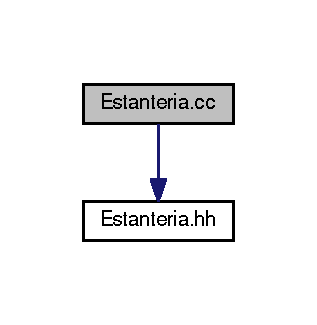
\includegraphics[width=152pt]{_estanteria_8cc__incl}
\end{center}
\end{figure}
\subsection*{Funcions}
\begin{DoxyCompactItemize}
\item 
bool \hyperlink{_estanteria_8cc_ac0047e8b44c74d982f8a9009e43c3e96}{cmp} (string \&A, string \&B)
\end{DoxyCompactItemize}


\subsection{Documentació de les Funcions}
\index{Estanteria.\+cc@{Estanteria.\+cc}!cmp@{cmp}}
\index{cmp@{cmp}!Estanteria.\+cc@{Estanteria.\+cc}}
\subsubsection[{\texorpdfstring{cmp(string \&\+A, string \&\+B)}{cmp(string &A, string &B)}}]{\setlength{\rightskip}{0pt plus 5cm}bool cmp (
\begin{DoxyParamCaption}
\item[{string \&}]{A, }
\item[{string \&}]{B}
\end{DoxyParamCaption}
)}\hypertarget{_estanteria_8cc_ac0047e8b44c74d982f8a9009e43c3e96}{}\label{_estanteria_8cc_ac0047e8b44c74d982f8a9009e43c3e96}


Definició a la línia 74 del fitxer Estanteria.\+cc.


\begin{DoxyCode}
74                                \{
75     \textcolor{keywordflow}{if} (A != \textcolor{stringliteral}{""} and B == \textcolor{stringliteral}{""}) \textcolor{keywordflow}{return} \textcolor{keyword}{true};
76     \textcolor{keywordflow}{else} \textcolor{keywordflow}{if} (A == \textcolor{stringliteral}{""} and B != \textcolor{stringliteral}{""}) \textcolor{keywordflow}{return} \textcolor{keyword}{false};
77     \textcolor{keywordflow}{else} \textcolor{keywordflow}{if} (A < B) \textcolor{keywordflow}{return} \textcolor{keyword}{true};
78     \textcolor{keywordflow}{return} \textcolor{keyword}{false};
79 \}
\end{DoxyCode}

\hypertarget{_estanteria_8hh}{}\section{Referència del Fitxer Estanteria.\+hh}
\label{_estanteria_8hh}\index{Estanteria.\+hh@{Estanteria.\+hh}}


Especificacio de la classe \hyperlink{class_estanteria}{Estanteria}.  


\subsection*{Classes}
\begin{DoxyCompactItemize}
\item 
class \hyperlink{class_estanteria}{Estanteria}
\begin{DoxyCompactList}\small\item\em Representa l\textquotesingle{}estanteria que hi ha a cada sala. \end{DoxyCompactList}\end{DoxyCompactItemize}


\subsection{Descripció Detallada}
Especificacio de la classe \hyperlink{class_estanteria}{Estanteria}. 


\hypertarget{_magatzem_8cc}{}\section{Referència del Fitxer Magatzem.\+cc}
\label{_magatzem_8cc}\index{Magatzem.\+cc@{Magatzem.\+cc}}
Inclou el graf de dependències per a Magatzem.\+cc\+:
\nopagebreak
\begin{figure}[H]
\begin{center}
\leavevmode
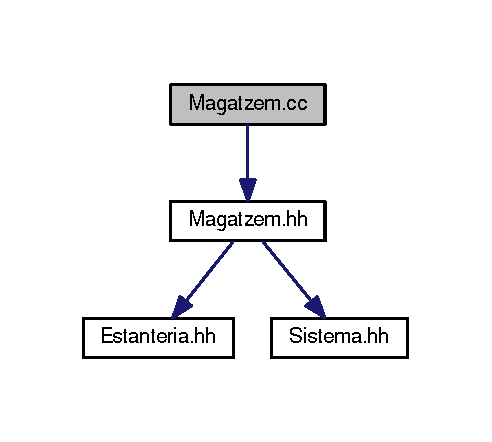
\includegraphics[width=236pt]{_magatzem_8cc__incl}
\end{center}
\end{figure}
\subsection*{Funcions}
\begin{DoxyCompactItemize}
\item 
void \hyperlink{_magatzem_8cc_a81091915104bc643983c4abb0ed3ab20}{llegir\+\_\+arbre} (Bin\+Tree$<$ int $>$ \&T, int \&nombre\+\_\+sales)
\item 
vector$<$ \hyperlink{class_estanteria}{Estanteria} $>$ \hyperlink{_magatzem_8cc_a7331a282952bdc8b18c070e57e5a13af}{llegir\+\_\+vector} (int \&nombre\+\_\+sales)
\end{DoxyCompactItemize}


\subsection{Documentació de les Funcions}
\index{Magatzem.\+cc@{Magatzem.\+cc}!llegir\+\_\+arbre@{llegir\+\_\+arbre}}
\index{llegir\+\_\+arbre@{llegir\+\_\+arbre}!Magatzem.\+cc@{Magatzem.\+cc}}
\subsubsection[{\texorpdfstring{llegir\+\_\+arbre(\+Bin\+Tree$<$ int $>$ \&\+T, int \&nombre\+\_\+sales)}{llegir_arbre(BinTree< int > &T, int &nombre_sales)}}]{\setlength{\rightskip}{0pt plus 5cm}void llegir\+\_\+arbre (
\begin{DoxyParamCaption}
\item[{Bin\+Tree$<$ int $>$ \&}]{T, }
\item[{int \&}]{nombre\+\_\+sales}
\end{DoxyParamCaption}
)}\hypertarget{_magatzem_8cc_a81091915104bc643983c4abb0ed3ab20}{}\label{_magatzem_8cc_a81091915104bc643983c4abb0ed3ab20}


Definició a la línia 65 del fitxer Magatzem.\+cc.


\begin{DoxyCode}
65                                                      \{
66     \textcolor{keywordtype}{int} n;
67     cin >> n;
68     \textcolor{keywordflow}{if} (n != 0 and n <= nombre\_sales) \{
69         BinTree<int> left;
70         BinTree<int> right;
71         \hyperlink{_magatzem_8cc_a81091915104bc643983c4abb0ed3ab20}{llegir\_arbre}(left,nombre\_sales);
72         \hyperlink{_magatzem_8cc_a81091915104bc643983c4abb0ed3ab20}{llegir\_arbre}(right,nombre\_sales);
73         T = BinTree<int>(n,left,right);
74     \}
75 \}
\end{DoxyCode}
\index{Magatzem.\+cc@{Magatzem.\+cc}!llegir\+\_\+vector@{llegir\+\_\+vector}}
\index{llegir\+\_\+vector@{llegir\+\_\+vector}!Magatzem.\+cc@{Magatzem.\+cc}}
\subsubsection[{\texorpdfstring{llegir\+\_\+vector(int \&nombre\+\_\+sales)}{llegir_vector(int &nombre_sales)}}]{\setlength{\rightskip}{0pt plus 5cm}vector$<${\bf Estanteria}$>$ llegir\+\_\+vector (
\begin{DoxyParamCaption}
\item[{int \&}]{nombre\+\_\+sales}
\end{DoxyParamCaption}
)}\hypertarget{_magatzem_8cc_a7331a282952bdc8b18c070e57e5a13af}{}\label{_magatzem_8cc_a7331a282952bdc8b18c070e57e5a13af}


Definició a la línia 77 del fitxer Magatzem.\+cc.


\begin{DoxyCode}
77                                                     \{
78     \textcolor{keywordtype}{int} i, j, k = 0;
79     vector<Estanteria> V (nombre\_sales);
80     \textcolor{keywordflow}{while} (k < nombre\_sales) \{
81         cin >> i >> j;
82         V[k] = \hyperlink{class_estanteria}{Estanteria}(i,j);
83         ++k;
84     \}
85     \textcolor{keywordflow}{return} V;
86 \}
\end{DoxyCode}

\hypertarget{_magatzem_8hh}{}\section{Referència del Fitxer Magatzem.\+hh}
\label{_magatzem_8hh}\index{Magatzem.\+hh@{Magatzem.\+hh}}


Especificacio de la classe \hyperlink{class_magatzem}{Magatzem}.  


Inclou el graf de dependències per a Magatzem.\+hh\+:
\nopagebreak
\begin{figure}[H]
\begin{center}
\leavevmode
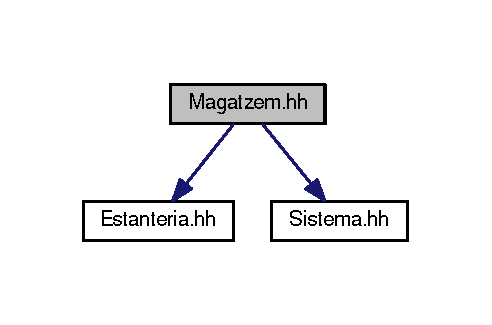
\includegraphics[width=236pt]{_magatzem_8hh__incl}
\end{center}
\end{figure}
\subsection*{Classes}
\begin{DoxyCompactItemize}
\item 
class \hyperlink{class_magatzem}{Magatzem}
\begin{DoxyCompactList}\small\item\em Representa un magatzem. \end{DoxyCompactList}\end{DoxyCompactItemize}


\subsection{Descripció Detallada}
Especificacio de la classe \hyperlink{class_magatzem}{Magatzem}. 


\hypertarget{program_8cc}{}\section{Referència del Fitxer program.\+cc}
\label{program_8cc}\index{program.\+cc@{program.\+cc}}
Inclou el graf de dependències per a program.\+cc\+:
\nopagebreak
\begin{figure}[H]
\begin{center}
\leavevmode
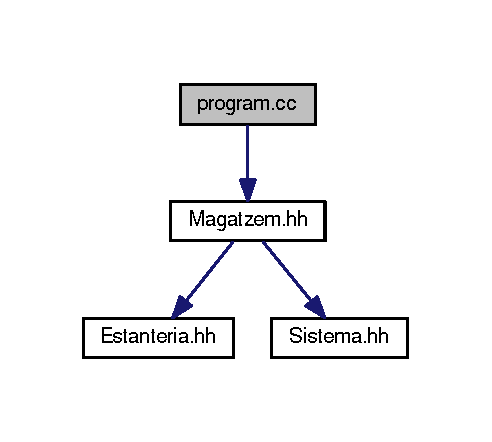
\includegraphics[width=236pt]{program_8cc__incl}
\end{center}
\end{figure}
\subsection*{Funcions}
\begin{DoxyCompactItemize}
\item 
int \hyperlink{program_8cc_ae66f6b31b5ad750f1fe042a706a4e3d4}{main} ()
\begin{DoxyCompactList}\small\item\em Programa principal de la simulacio del nou model de magatzem Tree\+K\+EA per a la cadena de tendes de mobles. \end{DoxyCompactList}\end{DoxyCompactItemize}


\subsection{Documentació de les Funcions}
\index{program.\+cc@{program.\+cc}!main@{main}}
\index{main@{main}!program.\+cc@{program.\+cc}}
\subsubsection[{\texorpdfstring{main()}{main()}}]{\setlength{\rightskip}{0pt plus 5cm}int main (
\begin{DoxyParamCaption}
{}
\end{DoxyParamCaption}
)}\hypertarget{program_8cc_ae66f6b31b5ad750f1fe042a706a4e3d4}{}\label{program_8cc_ae66f6b31b5ad750f1fe042a706a4e3d4}


Programa principal de la simulacio del nou model de magatzem Tree\+K\+EA per a la cadena de tendes de mobles. 



Definició a la línia 27 del fitxer program.\+cc.


\begin{DoxyCode}
27            \{
28     \hyperlink{class_magatzem}{Magatzem} Mag;
29     \textcolor{keywordtype}{int} num\_sales;
30     cin >> num\_sales;
31     Mag.\hyperlink{class_magatzem_acb77f36344a5cb8e5590487766400d1c}{llegir}(num\_sales);
32     \textcolor{keywordtype}{string} instruccio;
33     cin >> instruccio;
34     \textcolor{keywordflow}{while}(instruccio != \textcolor{stringliteral}{"fin"})\{
35             \textcolor{keywordflow}{if}(instruccio == \textcolor{stringliteral}{"consultar\_pos"})\{
36                     \textcolor{keywordtype}{int} idsala, f, c;
37                     cin >> idsala >> f >> c;
38                     cout << instruccio << \textcolor{stringliteral}{" "} << idsala << \textcolor{stringliteral}{" "} << f << \textcolor{stringliteral}{" "} << c << endl;
39                     Mag.\hyperlink{class_magatzem_a08da684e5a033414ccf05182b3993b5b}{consultar\_pos}(idsala,f,c);
40             \}
41             \textcolor{keywordflow}{else} \textcolor{keywordflow}{if}(instruccio == \textcolor{stringliteral}{"consultar\_prod"})\{
42                     \textcolor{keywordtype}{string} idprod;
43                     cin >> idprod;
44                     cout << instruccio << \textcolor{stringliteral}{" "} << idprod << endl;
45                     Mag.\hyperlink{class_magatzem_a0ce25c60c4ecb22acbc42836f160d770}{consultar\_prod\_en\_el\_s\_del\_mag}(idprod);
46             \}
47             \textcolor{keywordflow}{else} \textcolor{keywordflow}{if}(instruccio == \textcolor{stringliteral}{"inventario"})\{
48                     cout << instruccio << endl;
49                     Mag.\hyperlink{class_magatzem_a504a5bbe9daa97e89f55caef7e234a0d}{inventario\_del\_mag}();
50             \}
51             \textcolor{keywordflow}{else} \textcolor{keywordflow}{if}(instruccio == \textcolor{stringliteral}{"escribir"})\{
52                     \textcolor{keywordtype}{int} idsala;
53                     cin >> idsala;
54                     cout << instruccio << \textcolor{stringliteral}{" "} << idsala << endl;
55                     Mag.\hyperlink{class_magatzem_a00b0dca704cec9b018c7cbd2a77a583a}{escribir}(idsala);
56             \}
57             \textcolor{keywordflow}{else} \textcolor{keywordflow}{if}(instruccio == \textcolor{stringliteral}{"poner\_prod"})\{
58                     \textcolor{keywordtype}{string} idprod;
59                     cin >> idprod;
60                     cout << instruccio << \textcolor{stringliteral}{" "} << idprod << endl;
61                     Mag.\hyperlink{class_magatzem_ab8776250b582bb6b7b666e426d1820c1}{poner\_prod\_en\_el\_s\_del\_mag}(idprod);
62             \}
63             \textcolor{keywordflow}{else} \textcolor{keywordflow}{if}(instruccio == \textcolor{stringliteral}{"quitar\_prod"})\{
64                     \textcolor{keywordtype}{string} idprod;
65                     cin >> idprod;
66                     cout << instruccio << \textcolor{stringliteral}{" "} << idprod << endl;
67                     Mag.\hyperlink{class_magatzem_a98bf19f0ad6438d4a305bc9dc7a2670e}{quitar\_prod\_del\_s\_del\_mag}(idprod);
68             \}
69             \textcolor{keywordflow}{else} \textcolor{keywordflow}{if}(instruccio == \textcolor{stringliteral}{"poner\_items"})\{
70                     \textcolor{keywordtype}{int} idsala, quant;
71                     \textcolor{keywordtype}{string} idprod;
72                     cin >> idsala >> idprod >> quant;
73                     cout << instruccio << \textcolor{stringliteral}{" "} << idsala << \textcolor{stringliteral}{" "} << idprod << \textcolor{stringliteral}{" "} << quant << endl;
74                     \textcolor{keywordflow}{if} (Mag.\hyperlink{class_magatzem_a401014dc25c79a3b0abbe05e4419d757}{esta\_prod\_al\_mag}(idprod)) \{
75                         Mag.\hyperlink{class_magatzem_a82f901c8287586a33faa0f3c5030de11}{poner\_items}(idsala, idprod, quant);
76                     \}
77                     \textcolor{keywordflow}{else} cout << \textcolor{stringliteral}{"  error"} << endl;
78             \}
79             \textcolor{keywordflow}{else} \textcolor{keywordflow}{if}(instruccio == \textcolor{stringliteral}{"quitar\_items"})\{
80                     \textcolor{keywordtype}{int} idsala, quant;
81                     \textcolor{keywordtype}{string} idprod;
82                     cin >> idsala >> idprod >> quant;
83                     cout << instruccio << \textcolor{stringliteral}{" "} << idsala << \textcolor{stringliteral}{" "} << idprod << \textcolor{stringliteral}{" "} << quant << endl;
84                     \textcolor{keywordflow}{if} (Mag.\hyperlink{class_magatzem_a401014dc25c79a3b0abbe05e4419d757}{esta\_prod\_al\_mag}(idprod)) Mag.
      \hyperlink{class_magatzem_afb609e5a5d912a56b8ae4f8e985602f5}{quitar\_items}(idsala, idprod, quant);
85                     \textcolor{keywordflow}{else} cout << \textcolor{stringliteral}{"  error"} << endl;
86             \}
87             \textcolor{keywordflow}{else} \textcolor{keywordflow}{if}(instruccio == \textcolor{stringliteral}{"distribuir"})\{
88                     \textcolor{keywordtype}{int} quant;
89                     \textcolor{keywordtype}{string} idprod;
90                     cin >> idprod >> quant;
91                     cout << instruccio << \textcolor{stringliteral}{" "} << idprod << \textcolor{stringliteral}{" "} << quant << endl;
92                     \textcolor{keywordflow}{if} (Mag.\hyperlink{class_magatzem_a401014dc25c79a3b0abbe05e4419d757}{esta\_prod\_al\_mag}(idprod)) Mag.
      \hyperlink{class_magatzem_a15c31f32a673b7e3cf4443d03ace19a6}{distribuir}(idprod,quant);
93                     \textcolor{keywordflow}{else} cout << \textcolor{stringliteral}{"  error"} << endl;
94             \}
95             \textcolor{keywordflow}{else} \textcolor{keywordflow}{if}(instruccio == \textcolor{stringliteral}{"compactar"})\{
96                     \textcolor{keywordtype}{int} idsala;
97                     cin >> idsala;
98                     cout << instruccio << \textcolor{stringliteral}{" "} << idsala << endl;
99                     Mag.\hyperlink{class_magatzem_aeaebd6e73de2e965686264ecce7a0d26}{compactar}(idsala);
100             \}
101             \textcolor{keywordflow}{else} \textcolor{keywordflow}{if}(instruccio == \textcolor{stringliteral}{"reorganizar"})\{
102                     \textcolor{keywordtype}{int} idsala;
103                     cin >> idsala;
104                     cout << instruccio << \textcolor{stringliteral}{" "} << idsala << endl;
105                     Mag.\hyperlink{class_magatzem_a101e50b85da7acf8bfc892c03321c14c}{reorganizar}(idsala);
106             \}
107             \textcolor{keywordflow}{else} \textcolor{keywordflow}{if}(instruccio == \textcolor{stringliteral}{"redimensionar"})\{
108                     \textcolor{keywordtype}{int} idsala, f, c;
109                     cin >> idsala >> f >> c;
110                     cout << instruccio << \textcolor{stringliteral}{" "} << idsala << \textcolor{stringliteral}{" "} << f << \textcolor{stringliteral}{" "} << c << endl;
111                     Mag.\hyperlink{class_magatzem_adc1523fcbc1112437fdfe739fbeb393f}{redimensionar}(idsala,f,c);
112             \}
113             cin >> instruccio;  
114     \}
115     cout << \textcolor{stringliteral}{"fin"} << endl;
116 \}
\end{DoxyCode}

\hypertarget{_sistema_8cc}{}\section{Referència del Fitxer Sistema.\+cc}
\label{_sistema_8cc}\index{Sistema.\+cc@{Sistema.\+cc}}


Codi de la classe \hyperlink{_sistema_8cc}{Sistema.\+cc}.  


Inclou el graf de dependències per a Sistema.\+cc\+:
\nopagebreak
\begin{figure}[H]
\begin{center}
\leavevmode
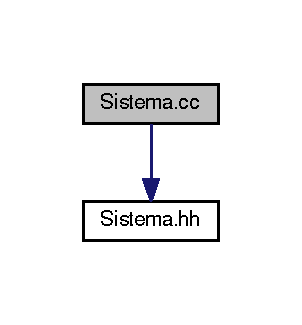
\includegraphics[width=145pt]{_sistema_8cc__incl}
\end{center}
\end{figure}


\subsection{Descripció Detallada}
Codi de la classe \hyperlink{_sistema_8cc}{Sistema.\+cc}. 


\hypertarget{_sistema_8hh}{}\section{Referència del Fitxer Sistema.\+hh}
\label{_sistema_8hh}\index{Sistema.\+hh@{Sistema.\+hh}}


Especificacio de la classe \hyperlink{class_sistema}{Sistema}.  


\subsection*{Classes}
\begin{DoxyCompactItemize}
\item 
class \hyperlink{class_sistema}{Sistema}
\begin{DoxyCompactList}\small\item\em Representa el sistema que controla els productes que hi ha dins del magatzem. \end{DoxyCompactList}\end{DoxyCompactItemize}


\subsection{Descripció Detallada}
Especificacio de la classe \hyperlink{class_sistema}{Sistema}. 


%--- End generated contents ---

% Index
\backmatter
\newpage
\phantomsection
\clearemptydoublepage
\addcontentsline{toc}{chapter}{Índex}
\printindex

\end{document}
